\documentclass{ieeeaccess}
\usepackage{cite}
\usepackage{amsmath,amssymb,amsfonts}
\usepackage{multirow}
\usepackage{algorithmic}
\usepackage{array}
\usepackage{makecell}
\usepackage[caption=false,font=normalsize,labelfont=sf,textfont=sf]{subfig}
\usepackage{textcomp}
\usepackage{url}
\usepackage{verbatim}
\usepackage{graphicx}

\usepackage{color}
\usepackage{framed}
\definecolor{revisionyellow}{rgb}{1,1,0}

\DeclareRobustCommand{\revinline}[1]{%
  \begingroup
  \setlength{\fboxsep}{1pt}%
  \colorbox{white}{\color{revisionred}\strut #1}%
  \endgroup
}

\DeclareRobustCommand{\revisioncaption}[1]{%
  \begingroup
  \setlength{\fboxsep}{1pt}%
  \colorbox{white}{\color{revisionred}%
    \parbox{0.82\linewidth}{\raggedright #1}%
  }%
  \endgroup
}

\newenvironment{revisionblock}
{%
  \par
  \begingroup
  \setlength{\fboxsep}{1pt}%
  \setlength{\OuterFrameSep}{0pt}%
  \def\FrameCommand##1{%
    \colorbox{white}{\color{revisionred}##1}%
  }%
  \MakeFramed{%
    \advance\hsize-2\fboxsep
    \FrameRestore
  }%
}
{%
  \endMakeFramed
  \endgroup
  \par
}
\usepackage{setspace}
\usepackage[switch]{lineno}
\linenumbers
\usepackage{subcaption}


\usepackage{pifont}
\newcommand{\circled}[1]{\textcircled{\scriptsize #1}}

\usepackage{balance}
\usepackage{bm}
\usepackage{booktabs}
\usepackage{float}
\usepackage{placeins}
\definecolor{RED}{rgb}{1,0,0}

\makeatletter
\AtBeginDocument{\DeclareMathVersion{bold}
\SetSymbolFont{operators}{bold}{T1}{times}{b}{n}
\SetSymbolFont{NewLetters}{bold}{T1}{times}{b}{it}
\SetMathAlphabet{\mathrm}{bold}{T1}{times}{b}{n}
\SetMathAlphabet{\mathit}{bold}{T1}{times}{b}{it}
\SetMathAlphabet{\mathbf}{bold}{T1}{times}{b}{n}
\SetMathAlphabet{\mathtt}{bold}{OT1}{pcr}{b}{n}
\SetSymbolFont{symbols}{bold}{OMS}{cmsy}{b}{n}
\renewcommand\boldmath{\@nomath\boldmath\mathversion{bold}}}
\makeatother

\def\BibTeX{{\rm B\kern-.05em{\sc i\kern-.025em b}\kern-.08em
    T\kern-.1667em\lower.7ex\hbox{E}\kern-.125emX}}

%Your document starts from here ___________________________________________________

% BEGIN REVISION STYLE: RED TEXT
\definecolor{revisionred}{RGB}{190,0,0}

\providecommand{\revinline}[1]{#1}
\renewcommand{\revinline}[1]{{\color{revisionred}#1}}

\providecommand{\revisioncaption}[1]{#1}
\renewcommand{\revisioncaption}[1]{{\color{revisionred}#1}}

\providecommand{\revisioncaptioncompact}[1]{#1}
\renewcommand{\revisioncaptioncompact}[1]{{\color{revisionred}#1}}

\renewenvironment{revisionblock}
  {\par\begingroup\color{revisionred}}
  {\par\endgroup}
% END REVISION STYLE: RED TEXT

\begin{document}
\history{Date of publication xxxx 00, 0000, date of current version xxxx 00, 0000.}
\doi{10.1109/ACCESS.2024.0429000}

\title{Comparative Evaluation of Deep Neural Network Architectures for Loop Closure Detection in Visual SLAM}

\author{Fabiana Naomi Iegawa\authorrefmark{1}, Wagner Tanaka Botelho\authorrefmark{1}, Flavio Shigeo Yamamoto\authorrefmark{2}, Fábio Suim Chagas\authorrefmark{3}, Marlon M. López-Flores\authorrefmark{4} and Paulo Fernando Ferreira Rosa\authorrefmark{4}}

\address[1]{Federal University of ABC, Centre os Mathematics, Computation and Cognition, Santo André, São Paulo - SP, Brazil (e-mail: wagner.tanaka@ufabc.edu.br)}
\address[2]{Startup NTU Software Technology, São Paulo, São Paulo - SP, Brazil}
\address[3]{Department of Design, Norwegian University of Science and Technology, Skippergata, 14 7042 Trondheim, Norway}
\address[4]{Laboratory for Artificial Intelligence, Robotics and Cybernetics - LIARC, Military Institute of Engineering - IME-RJ, Rio de Janeiro, Brazil}
\tfootnote{The authors would like to thank the São Paulo Research Foundation (FAPESP) for financial support under Grant No. 2015/02301-3 and for the TT-3 research fellowship (Grant No. 2019/12080-5), funded through the FAPESP/PIPE Program and provided by NTU Software Technology (Grant No. 2018/04306-0) from July 2019 to December 2020. This work was also partially supported by the Artificial Intelligence, Robotics, and Cybernetics Laboratory at the Instituto Militar de Engenharia, Rio de Janeiro, RJ, Brazil, and by Project EVAAT\_GCN (FINEP Grant No. 01.24.0661.00 - 3311/24).}

\markboth
{Author \headeretal: Preparation of Papers for IEEE TRANSACTIONS and JOURNALS}
{Author \headeretal: Preparation of Papers for IEEE TRANSACTIONS and JOURNALS}

\corresp{Corresponding author: Wagner Tanaka Botelho (e-mail: wagner.tanaka@ufabc.edu.br).}

\begin{abstract}
Loop Closure Detection is a fundamental component of Visual Simultaneous Localization and Mapping (SLAM), as it enables the recognition of previously visited locations and mitigates localization drift and map inconsistencies. However, robust Loop Closure Detection remains challenging under viewpoint changes, illumination variations, opposite traversal directions, and camera rotations. This paper presents a systematic and reproducible framework for evaluating deep visual descriptors under diverse operational conditions. Using the KITTI and TUM datasets, multiple Deep Neural Networks (DNNs) architectures are comparatively analyzed, including AlexNet, ConvNeXt, ResNet, Original VGG-16, Adapted and Fine-Tuned VGG-16, and Vision Transformer (ViT). The proposed framework investigates descriptor extraction and image-matching strategies for Visual SLAM place recognition. Performance is assessed using Accuracy, F1-score, Receiver Operating Characteristic (ROC) curves, and Area Under the Curve (AUC). Experimental results show that descriptor performance is highly dependent on viewpoint variation, traversal direction, and camera rotation. The Adapted and Fine-Tuned VGG-16 achieved the best results under relatively stable viewpoint conditions, whereas ResNet demonstrated comparatively stronger robustness in the evaluated opposite-traversal scenario. These findings highlight the strong influence of representation-learning strategies and operational conditions on Loop Closure Detection performance.
\end{abstract}

\begin{keywords}
Visual SLAM, Loop Closure Detection, Visual Place Recognition, Deep Visual Descriptors, Convolutional Neural Networks, Vision Transformers.
\end{keywords}

\titlepgskip=-21pt

\maketitle

\section{Introduction} 

Accurate localization and consistent map creation are fundamental requirements for autonomous robot navigation. However, both are often degraded by error accumulation from sensor noise, uncertainties in motion estimation, and long-term drift in real-world environments. Consequently, the estimated robot pose may progressively deviate from the true trajectory, degrading map quality, impairing trajectory planning, and reducing the reliability of autonomous decision-making. In the Simultaneous Localization and Mapping (SLAM) paradigm, Loop Closure Detection is a key technique for addressing this issue by recognizing previously visited locations and correcting localization and mapping errors \cite{Cadena2016SLAM,DurrantWhyte2006SLAMPartI,Thrun2008SLAM,Chen2020SurveyDeepLearningLocalizationMapping}.

Loop Closure Detection is a critical mechanism of SLAM, particularly in visual systems, because navigation without reliable Loop Closure relies heavily on odometric propagation. Consequently, previously visited regions may be misclassified as unexplored, resulting in globally inconsistent maps and inaccurate pose estimation. By recognizing that the robot has returned to a previously mapped location, Loop Closure enables joint correction of pose estimates and map representations, thereby preserving spatial consistency and improving navigation robustness \cite{Cadena2016SLAM,Taketomi2017VisualSLAMSurvey,Williams2009LoopClosingComparison}. Reliable Loop Closure Detection significantly improves localization consistency, map quality, and long-term autonomous navigation performance \cite{Lowry2016,Arshad2021}. Furthermore, \cite{Xu2022SiameseConvNetRGBDSLAM} highlighted that Loop Closure Detection remains one of the main challenges in Visual SLAM systems, which has motivated increasing research interest in recent years.

In Visual SLAM, Loop Closure Detection is closely related to the visual place recognition problem. However, reliable place recognition remains challenging under viewpoint variations, illumination changes, dynamic environments, perceptual aliasing, and opposite traversal directions. These conditions frequently produce false positives and false negatives, directly affecting localization accuracy and map consistency. Moreover, large-scale environments introduce additional computational constraints due to the need for real-time descriptor matching against extensive image databases \cite{Lowry2016,Garg2018DontLookBack,Naseer2014NetworkFlowsSeasons,Arshad2021,Wang2024SemanticLineGraphLoopClosure}. According to \cite{AliBey2023MixVPR} and \cite{Wang2024SemanticLineGraphLoopClosure}, at scale, repetitive patterns, viewpoint changes, weather variations, and lighting changes pose significant challenges because appearances can vary substantially over time.

Traditional Loop Closure Detection approaches rely primarily on handcrafted local descriptors and geometric verification techniques. Classical methods such as Scale-Invariant Feature Transform (SIFT) \cite{Lowe2004SIFT}, Speeded-Up Robust Features (SURF) \cite{Bay2006SURF}, and Oriented FAST and Rotated BRIEF (ORB) \cite{Campos2021ORBSLAM3} played a key role in developing robust Visual SLAM pipelines, including ORB-SLAM-based systems \cite{MurArtal2017ORBSLAM2,Campos2021ORBSLAM3}. Despite their effectiveness, handcrafted descriptors often lose discriminative power under severe appearance changes and viewpoint variations, limiting robustness in real-world environments \cite{Lowry2016,Arshad2021}. 

With the rapid advancement of Deep Learning in Computer Vision, particularly in object recognition and image classification, Deep Neural Networks (DNNs) have increasingly been explored for Loop Closure Detection tasks \cite{Ng2015LocalDeepFeaturesImageRetrieval}. \cite{Chen2025PanoramicSemanticTopologicalMap} proposed a 3D panoramic semantic topological map that integrates semantic, depth, and spatial information to improve Loop Closure recognition.

Recent advances in deep architectures have significantly improved visual representation learning for place recognition and Loop Closure Detection. Convolutional Neural Networks (CNNs) and Transformer-based architectures have demonstrated improved robustness in prior studies to complex appearance variations, enabling more discriminative and semantically rich visual descriptors \cite{Sunderhauf2015ConvNetPlaceRecognition,Chen2019,AliBey2023MixVPR,Chen2025PanoramicSemanticTopologicalMap}. As a result, deep learning-based approaches have become increasingly relevant to robust Visual SLAM systems.

Despite recent advances, several challenges remain in Deep Learning-based Loop Closure Detection systems. Perceptual aliasing, dynamic environments, viewpoint variation, and appearance changes continue to compromise descriptor robustness and matching reliability \cite{Chen2019,Wang2024SemanticLineGraphLoopClosure}. In addition, balancing recognition accuracy and computational efficiency remains critical for real-time operation in large-scale environments \cite{Arshad2021}. Furthermore, comparative evidence on the robustness of CNN- and Transformer-based visual descriptors under heterogeneous operational conditions, such as opposite traversal directions and camera rotations, remains limited.

In this context, this paper presents a systematic, reproducible evaluation of deep visual descriptors for Loop Closure Detection across varying operational conditions, using the KITTI \cite{Geiger2013KITTI} and TUM \cite{Sturm2012RGBDSLAMBenchmark} datasets. The study assesses descriptor robustness to viewpoint changes, opposite traversal directions, and camera rotations, using the architectures AlexNet \cite{Krizhevsky2017AlexNetCACM}, ConvNeXt \cite{Liu2022ConvNeXt}, ResNet \cite{He2016ResNet}, Original VGG-16 \cite{Simonyan2015VGG}, Adapted and Fine-Tuned VGG-16, and Vision Transformer (ViT) \cite{Dosovitskiy2021ViT}. Performance is evaluated using Accuracy, F1-score, Receiver Operating Characteristic (ROC) curves, and Area Under the Curve (AUC).

Except for the Adapted and Fine-Tuned VGG-16, all evaluated models are publicly available in the PyTorch ecosystem and widely used for image classification. The Adapted and Fine-Tuned VGG-16 proposed in \cite{Iegawa2023LoopClosureCNN} was obtained by fine-tuning the Original VGG-16 architecture. The present work extends the experimental evaluation presented in \cite{Iegawa2023LoopClosureCNN}, which focused exclusively on a single Fine-Tuned VGG-16 architecture evaluated in simulated environments. In contrast, the current study presents a comparative evaluation of multiple CNN- and Transformer-based architectures using public datasets, including ROC/AUC analysis, confusion matrices, and robustness assessment under viewpoint variation, opposite traversal directions, and camera rotation. Therefore, the main objective of this paper is to evaluate the robustness of deep visual descriptors for Loop Closure Detection under challenging operational conditions.

Based on the challenges and limitations identified in the literature, this work provides the following contributions: a systematic, reproducible evaluation framework for deep visual descriptors in Loop Closure Detection, along with an experimental analysis of descriptor robustness to viewpoint changes, opposite traversal directions, and camera rotations across the KITTI and TUM public datasets. The work also presents a comparative evaluation of CNN- and Transformer-based architectures and validates an Adapted and Fine-Tuned VGG-16 architecture for Loop Closure Detection in Visual SLAM scenarios. The framework uses publicly available datasets, pretrained models, and standardized evaluation metrics to facilitate reproducibility. Finally, all materials created and used in this work, including code, simulation videos, datasets, and other files, are available at \cite{IegawaBotelho2022LoopClosureGitHub}. 

The remainder of this paper is organized as follows. Section \ref{sec:Related} reviews related work on Loop Closure Detection. Section \ref{sec:Loop} presents the explored evaluation framework. Section \ref{sec:resul} discusses the results. Finally, Section \ref{sec:concl} concludes the paper and outlines directions for future work.

\section{Related Work}
\label{sec:Related}

Early Loop Closure Detection approaches relied primarily on handcrafted local descriptors and probabilistic SLAM formulations. Although effective in some scenarios, these methods are computationally expensive and often unsuitable for real-time Visual SLAM in large-scale environments \cite{Arshad2021}.

SIFT, investigated in \cite{Lowe2004SIFT}, was among the earliest feature descriptors used for Loop Closure Detection. It detects and describes local image features in a scale-invariant manner. In \cite{Ali2010SIFTMonocularSLAM}, SIFT features were extracted from monocular images to build a feature representation for indoor navigation, yielding accurate pose estimates and object identification rates above 50\%. To generate rotation- and scale-invariant descriptors more efficiently, \cite{Bay2006SURF} introduced SURF. Although computationally less expensive than SIFT, SURF was less robust to illumination variations. ORB-SLAM, developed in \cite{Naseer2015RobustVisualSLAMAcrossSeasons}, is widely regarded as one of the most robust Visual SLAM systems. Using ORB features enabled real-time operation and improved tolerance to illumination changes during data association.

With advances in Deep Learning, visual place recognition and Loop Closure Detection increasingly rely on learned visual representations. Both supervised and unsupervised learning strategies have been explored to improve Visual SLAM robustness and localization performance, as discussed in \cite{Kazerouni2022VisualSLAMSurvey}. In addition, \cite{Song2025VSSLAM} introduced a LiDAR-based SLAM framework that uses virtual descriptors to identify previously visited locations even when trajectories do not exactly overlap. \cite{zhou2025siamesecapsule} explored a lightweight siamese capsule network for Loop Closure Detection, improving descriptor robustness while reducing computational complexity.

Many Deep Learning-based Loop Closure Detection approaches use architectures originally designed for object recognition and image classification. However, unlike object-centric applications, visual place recognition requires robust global scene understanding to handle severe appearance and viewpoint variations. In contrast, \cite{wang2023hybrid} investigated a robust and efficient Loop Closure Detection approach for hybrid ground/aerial vehicles, aiming to improve robustness under heterogeneous viewpoints.

\cite{Chen2025PanoramicSemanticTopologicalMap} proposed a Generative Adversarial Network (GAN)-based framework that extracts features from the network's discriminator. The network was trained, and the discriminator's final feature layer was used to detect Loop Closure. A similarity matrix was also used to compare descriptors and identify previously observed images. To compare descriptors extracted from different network layers, \cite{Ng2015LocalDeepFeaturesImageRetrieval} used VGG-16 \cite{Simonyan2015VGG} and GoogLeNet \cite{Szegedy2015GoogLeNet} to extract image features. To improve the efficiency of image similarity search, the authors adopted the Vector of Locally Aggregated Descriptors (VLAD) framework \cite{Jegou2010VLAD}, which represents an image by aggregating local descriptors into compact visual representations. The outputs of convolutional layers were aggregated into compact descriptor vectors, and descriptors extracted from intermediate layers achieved better image association performance.

\cite{Chen2017OnlyLookOnce} introduced an additional convolutional layer to extract features and used deeper activations to identify salient image regions. Seasonal appearance changes in outdoor environments make Loop Closure Detection particularly challenging. To address this challenge, \cite{Naseer2015RobustVisualSLAMAcrossSeasons} extracted features from two image sequences captured in different seasons, using CNN architectures based on GoogLeNet \cite{Szegedy2015GoogLeNet} and AlexNet \cite{Krizhevsky2017AlexNetCACM}. The descriptors from the two sequences were used to create a similarity matrix and compare all images. The authors combined odometry information with the similarity matrix to formulate a graph-based SLAM system. \cite{Bai2016MatchingRangeCNNLoopClosure} investigated Places-CNN features and reported false matches between adjacent images in Loop Closure Detection. 

Graph-based autoencoder approaches have also been explored to preserve local geometric consistency during descriptor learning. The developed G-Stacked Denoising Autoencoder (SDAE) incorporated graph regularization to learn local geometric structures and generate descriptors for Loop Closure Detection \cite{Vincent2010StackedDenoisingAutoencoders,Wang2019GraphAutoEncoderLoopClosure}. More recently, variational autoencoder (VAE)-based approaches have been investigated for Loop Closure Detection in Visual SLAM. \cite{song2024vae} explored a VAE-based framework that learns compact latent representations to improve robustness to appearance variations and viewpoint changes.

In \cite{Memon2020DeepLoopClosure}, supervised and unsupervised learning methods were combined to detect Loop Closure. A CNN-based classifier extracted semantic scene information, and an autoencoder identified previously unseen environments and was retrained online. A super dictionary and a key-frame dictionary were introduced to accelerate image comparison and reduce false positives. \cite{jiang2024compressed} proposed a Loop Closure Detection method based on compressed ConvNet features to improve computational efficiency and robustness in dynamic environments.

Despite substantial progress, the literature still lacks systematic, reproducible comparative studies that evaluate CNN- and Transformer-based visual descriptors under unified operational conditions. In particular, limited attention has been given to the combined effects of viewpoint variation, opposite traversal directions, and camera rotations on descriptor robustness in Visual SLAM environments. These gaps underscore the need for the evaluation framework investigated in this paper. Another important limitation in the literature is the lack of standardized evaluation protocols across datasets and operational conditions, making direct comparisons between methods difficult.

\section{Proposed Evaluation Framework}
\label{sec:Loop}

This section presents the proposed experimental framework for evaluating deep visual descriptors for Loop Closure Detection across varying operational conditions.

Fig. \ref{fig:Fig1} illustrates the investigated evaluation framework for \circled{1} Loop Closure Detection using \circled{2} DNN Architectures. The (a) Environment is represented by public datasets of real-world outdoor images, such as KITTI \cite{Geiger2013KITTI} and TUM \cite{Sturm2012RGBDSLAMBenchmark}. During (b) Preprocessing, images are split into left and right regions to improve robustness to traversal direction, following the strategy proposed in \cite{Garg2018DontLookBack}. In the (c) Feature Extraction, models such as (d) AlexNet \cite{Krizhevsky2017AlexNetCACM}, (e) ConvNeXt \cite{Liu2022ConvNeXt}, (f) ResNet \cite{He2016ResNet}, (g) Original VGG-16 \cite{Simonyan2015VGG}, (h) Adapted and Fine-Tuned VGG-16 \cite{Iegawa2023LoopClosureCNN}, and (j) Vision Transformer \cite{Dosovitskiy2021ViT} are used for (k) Descriptor Generation.

\begin{figure*}[!t]
	\centering
	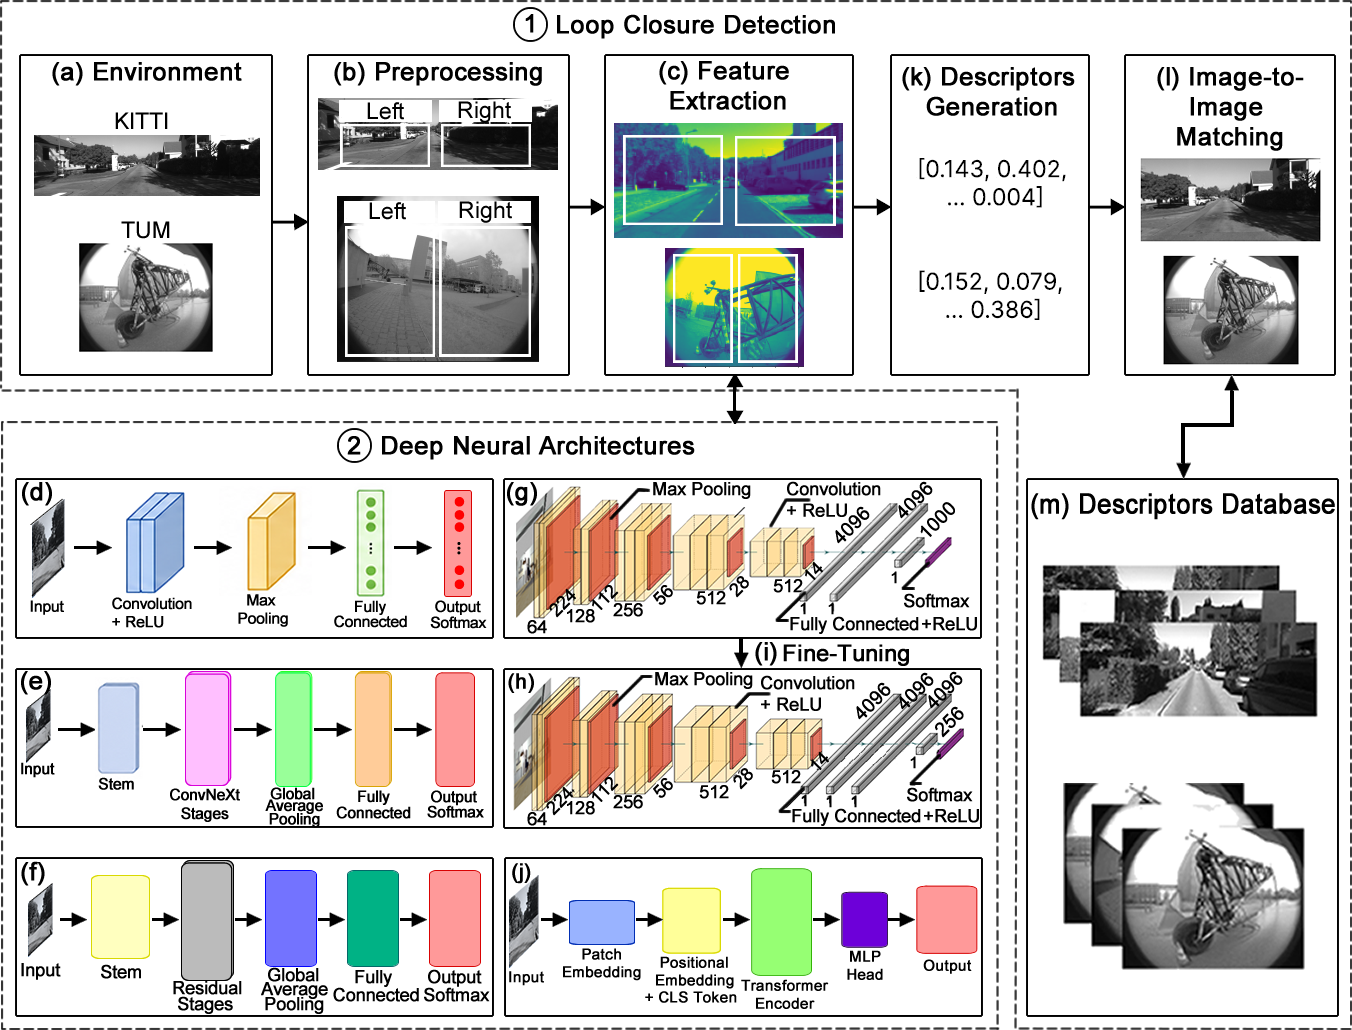
\includegraphics[width=\linewidth]{./Figures/Fig_1.png}
	\caption{Steps to Detect the Loop Closure.}
	\label{fig:Fig1}
\end{figure*}

\subsection{Loop Closure Detection}

Fig. \ref{fig:fechamento} details the processing pipeline of the proposed evaluation framework. Images from the  \circled{1} Environment are resized, normalized, and converted into tensors in the \circled{2} Preprocessing before \circled{3} Feature Extraction. In the \circled{3}, features such as corners and object edges are extracted and used for \circled{4} Descriptors Generation. Lastly, the \circled{5} Image-to-Image Matching is applied to detect Loop Closure candidates. 

\begin{figure}[!t]
	\centering
	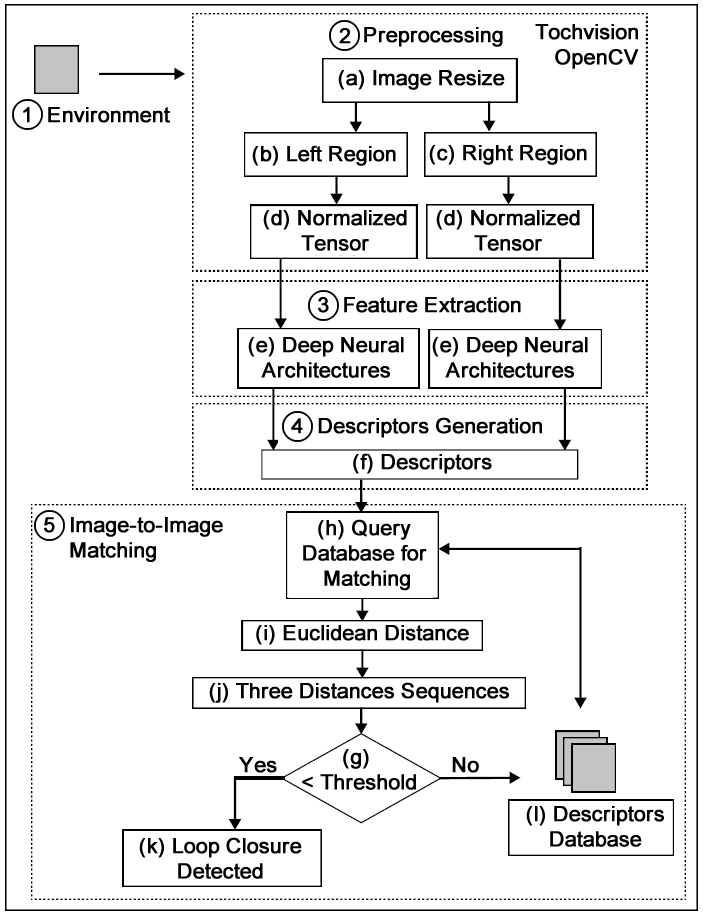
\includegraphics[width=\linewidth]{./Figures/Fig_2.png}
	\caption{Loop Closure Detection Pipeline, Adapted and Extended from \cite{Iegawa2023LoopClosureCNN}.}
	\label{fig:fechamento}
\end{figure}

\vspace{0.3cm}
\noindent
\emph{\textbf{Environment and Preprocessing}}
\vspace{0.3cm}

The Scenario shown in Fig. \ref{fig:Fig1} (a) and Fig. \ref{fig:fechamento} \circled{1} displays images from the public datasets KITTI and TUM. In the Preprocessing, illustrated in Figs. \ref{fig:Fig1} (b) and \ref{fig:fechamento} \circled{2}, the (a) Resize Image receives the image from step \circled{1} as input, resizes it to $540$ x $540$ pixels, and splits it into two parts: (b) Left Region and (c) Right Region. According to \cite{Garg2018DontLookBack}, splitting the image may improve robustness in recognizing a two-point path when revisited in reverse order. Moreover, after the division, each image region is converted into (d) Normalized Tensor using the Torchvision preprocessing pipeline. The images are resized and normalized according to the input requirements of the evaluated DNN architectures. This (b) Preprocessing step helps standardize the input distribution and standardizes the data before feature extraction.

\vspace{0.3cm}
\noindent
\emph{\textbf{Feature Extraction and Descriptor Generation}}
\vspace{0.3cm}

Relevant scenario information is detected and extracted during Feature Extraction, as illustrated in Fig. \ref{fig:Fig1}(c) and Fig.  \ref{fig:fechamento} \circled{3}. The (d) Normalized Tensor is processed by the selected (e) Deep Neural Architectures, and the output of the penultimate network layer is used for Loop Closure Detection. As shown in Fig. \ref{fig:Fig1}, the (e) considered in this study include (d) AlexNet, (e) ConvNeXt, (f) ResNet, the (g) Original VGG-16, the (h) Adapted and Fine-Tuned VGG-16 - (i) Fine-Tuning, and the (j) Vision Transformer. In each architecture, successive layers extract increasingly abstract visual representations that are propagated to subsequent layers. Therefore, the output of a given layer may be selected as the feature representation for Loop Closure Detection.

In Fig. \ref{fig:Fig1} (k) and Fig. \ref{fig:fechamento} \circled{4}, descriptors are generated by concatenating feature tensors obtained after \circled{3} Feature Extraction, from left to right. The final tensor is called (f) Descriptors. This step captures complementary spatial information from both image regions by considering the features of the two regions within a single sequence to improve Loop Closure Detection robustness.

\vspace{0.3cm}
\noindent
\emph{\textbf{Image-to-Image Matching and Descriptor Database}}
\vspace{0.3cm}

Before the Image-to-Image Matching in Fig. \ref{fig:Fig1} (l) and Fig. \ref{fig:fechamento} \circled{5}, the matching (g) Threshold is empirically estimated using reference image pairs acquired under controlled operational conditions. Euclidean distances are computed between descriptors extracted from matching image pairs, and an empirically defined descriptor distance threshold is used to set the operational matching threshold for binary Loop Closure Detection. To prevent data leakage, the image pairs used for threshold estimation were excluded from the final Loop Closure evaluation protocol. This operational threshold is independent of the ROC analysis, since the ROC curves were generated by sweeping multiple descriptor distance thresholds exclusively for performance evaluation, not for operational decision-making.

The operational thresholds were estimated independently for each evaluated neural architecture and dataset using reference image pairs acquired separately from the final evaluation samples. For threshold estimation, a control image was selected, and additional images of the same environment were captured under variations in illumination and viewpoint. Euclidean distances between descriptor pairs were computed, and the average descriptor distance was used to define the operational threshold for each experimental condition.

The Image-to-Image Matching step, shown in Fig. \ref{fig:Fig1} (l) and Fig. \ref{fig:fechamento} \circled{5}, aims to detect Loop Closure candidates while minimizing false positives. First, using the (f) Descriptors of \circled{1} Environment, one must (h) Query Database for Matching and select all images in descriptor format to find Loop Closure candidates. Then, the (i) Euclidean Distance between the Scenario (f) Descriptors of the images consulted in (h) is calculated. The (i) represents the difference between the images, calculated in tensor form, and its maximum value is used to create the (j) Three Distance Sequences. Accordingly, only the maximum distances are grouped into sets of three, reducing computational overhead. 

For the (j) Three Distance Sequences shown in Fig. \ref{fig:fechamento}, each Euclidean distance within the three-descriptor sequence is compared with the threshold, which indicates the maximum difference between descriptors for two images to be considered similar. If all sequence values in (j) are less than those in (g), the result is (k) Loop Closure Detected. Otherwise, the descriptors should be stored in the (l) Descriptors Database for further comparisons. The sequences in (j) ensure that a sequence is observed, preventing false positives in which only one or two of the distances in (i) are under (g). Therefore, this strategy introduces temporal consistency into Loop Closure Detection, reducing isolated false positives.

\subsection{Deep Neural Architectures}

This paper evaluates deep visual descriptors extracted from multiple \circled{2} Deep Neural Architectures, shown in Fig. \ref{fig:Fig1}, across different representation paradigms, including classical CNN architectures, modern convolutional architectures, and Transformer-based models. Rather than emphasizing image classification accuracy, the analysis investigates descriptor robustness for Loop Closure Detection on the KITTI and TUM datasets. Because each neural architecture generates descriptor vectors with distinct dimensionalities and statistical distributions, threshold calibration was performed independently for each evaluated model.

In Fig. \ref{fig:Fig1}, the evaluated \circled{2} Deep Neural Architectures are (d) AlexNet \cite{Krizhevsky2017AlexNetCACM}, (e) ConvNeXt \cite{Liu2022ConvNeXt}, (f) ResNet \cite{He2016ResNet}, (g) Original VGG-16 \cite{Simonyan2015VGG}, (h) Adapted and Fine-Tuned VGG-16 \cite{Iegawa2023LoopClosureCNN}, and (j) Vision Transformer \cite{Dosovitskiy2021ViT}. Except for (h) Adapted and Fine-Tuned VGG-16, all architectures are available in the PyTorch ecosystem and were pretrained on ImageNet.

For each architecture, descriptors are extracted from high-level semantic representation layers, enabling a systematic comparison of the semantic visual representations produced by different Deep Learning paradigms. Table \ref{tab:descriptor_architectures} summarizes the evaluated architectures, the layers selected for descriptor extraction, descriptor dimensionality, and the representation types used in the explored evaluation framework, as illustrated in Figs. \ref{fig:Fig1} and \ref{fig:fechamento}.

\begin{table}[!t]
\centering
\caption{DNN Architectures Evaluated in the Proposed Framework.}
\label{tab:descriptor_architectures}
\renewcommand{\arraystretch}{1.15}

\resizebox{\columnwidth}{!}{
\begin{tabular}{|m{2.2cm}|m{3.0cm}|m{1.8cm}|m{2.0cm}|}
\hline

\multicolumn{1}{|c|}{\textbf{Architecture}} &
\multicolumn{1}{c|}{\textbf{Feature Layer}} &
\multicolumn{1}{c|}{\begin{tabular}[c]{@{}c@{}}\textbf{Feature}\\ \textbf{Dimension}\end{tabular}} &
\multicolumn{1}{c|}{\textbf{Model Type}} \\

\hline

AlexNet &
Last Fully Connected Layer (FC7) &
\centering 4096 &
Classical CNN \\

\hline

ConvNeXt &
Final Convolutional Block &
\centering 768 &
Modern CNN \\

\hline

ResNet &
Last Convolutional Layer &
\centering 2048 &
Residual CNN \\

\hline

Original VGG-16 &
Fully Connected Layer (FC2) &
\centering 4096 &
CNN \\

\hline

Adapted and Fine-Tuned VGG-16 &
Final Fully Connected Layer &
\centering 256 &
Fine-Tuning CNN \\

\hline

Vision Transformer &
Final Fully Connected Layer &
\centering 768 &
\begin{tabular}[c]{@{}c@{}}Transformer\end{tabular} \\

\hline

\end{tabular}
}
\end{table}

As shown in Table \ref{tab:descriptor_architectures}, AlexNet \cite{Alom2018HistoryBeganAlexNet, Krizhevsky2017AlexNetCACM} is evaluated as a classical CNN baseline for visual descriptor extraction. ResNet \cite{He2016ResNet} and ConvNeXt \cite{Liu2022ConvNeXt} are included to investigate the descriptor robustness of modern convolution-based representations under viewpoint variations and opposite traversal directions. The Vision Transformer \cite{Vaswani2017Attention, Guo2022ExternalAttention,Dosovitskiy2021ViT} is evaluated to analyze the behavior of global Transformer-based feature representations in Loop Closure Detection scenarios.

The (g) VGG-16 model shown in Fig. \ref{fig:Fig1}, referred to (g) Original VGG-16, details each layer and its corresponding output dimensions. It consists of convolutional and fully connected layers that progressively extract hierarchical visual representations. However, the (h) Adapted and Fine-Tuned VGG-16 architecture, also presented in Table \ref{tab:descriptor_architectures}, was derived from the (g) through (i) Fine-Tuning and was previously proposed by \cite{Iegawa2023LoopClosureCNN}. In the (h), the convolutional layers were kept frozen during retraining. Additional fully connected layers were introduced,
and the third layer was replaced by two fully connected layers with $4096$ and $256$ dimensional outputs, respectively. The final layers were trained to enhance activations in the fully connected layers.  According to \cite{Iegawa2023LoopClosureCNN}, these final layers were trained using virtual images generated in the Gazebo simulator to reduce descriptor dimensionality and improve robustness during feature extraction for Loop Closure Detection. Consequently, this architecture is included in the proposed evaluation framework to investigate whether task-specific adaptation improves descriptor robustness under challenging operational conditions, particularly in scenarios involving camera rotations and opposite traversal directions. 

Because Loop Closure Detection is an imbalanced classification problem, Accuracy alone may not adequately represent descriptor matching performance. Therefore, the evaluation also considers F1-score, ROC curves, and AUC. ROC curves were generated by sweeping multiple thresholds across the continuous descriptor similarity scores, enabling analysis of TPR and FPR under different decision boundaries.



\subsection{\revinline{Reproducible ResNet-101 L=1 Audit}}
\label{sec:resnet_l1_audit}

\begin{revisionblock}
A focused reproducibility audit was additionally conducted for ResNet-101 on KITTI odometry sequence 05 at the descriptor level ($L=1$), independently from the three-distance temporal verification described above. The 2,761 frames from the left grayscale camera (\texttt{image\_0}) were processed in their original order. Each frame was resized to $256 \times 256$ pixels, normalized using mean $0.36$ and standard deviation $0.28$, and divided into two $124 \times 124$ crops. The left crop started at $(4,4)$ and the right crop at $(4,124)$ in $(\mathrm{top},\mathrm{left})$ coordinates. A ResNet-101 model with explicit ImageNet-1K V1 pretrained weights was executed in evaluation and inference modes. The 2,048-dimensional average-pooling outputs produced for the two crops were concatenated into a 4,096-dimensional descriptor.

Two descriptor-distance formulations were evaluated. The reconstructed legacy formulation was
\begin{equation}
d_{\infty}(\mathbf{q},\mathbf{r})
=
\max_i |q_i-r_i|,
\end{equation}
which corresponds to the maximum absolute descriptor-component difference. The corrected formulation used the flattened Euclidean distance
\begin{equation}
d_2(\mathbf{q},\mathbf{r})
=
\sqrt{\sum_i (q_i-r_i)^2}.
\end{equation}
Continuous similarity scores were defined as $s=-d$, so larger scores indicate more similar descriptors. This distinction is important because applying a maximum operation after the reconstructed tensor-distance computation does not yield a conventional flattened Euclidean distance.

Candidate pairs were assigned to the positive class when their spatial separation was at most $5$ m, to an ambiguous interval when it was greater than $5$ m and less than $10$ m, and to the negative class when it was at least $10$ m. Ambiguous pairs were retained in the generated score files for auditability but excluded from binary metrics. Three independent revisit events were used as calibration, test, and stress splits. For each distance formulation, the operational threshold was selected exclusively on the calibration event by maximizing the F1-score and was then applied without recalibration to the test and stress events. Ranking performance was reported using ROC-AUC, precision--recall AUC (PR-AUC), and Average Precision (AP), whereas F1-score and the confusion matrix characterized the fixed calibration-derived operating point. These $L=1$ descriptor results are intentionally separated from temporal verification experiments, which require an explicit analysis over sequence lengths such as $L\in\{1,2,3,5\}$.
\end{revisionblock}

\section{Results and Discussion} 
\label{sec:resul}

This section presents the experimental evaluation and discusses the robustness of deep visual descriptors for Loop Closure Detection across distinct operational conditions, using the KITTI and TUM datasets. The architectures evaluated, illustrated in Fig. \ref{fig:Fig1}, include AlexNet, ConvNeXt, ResNet, Original VGG-16, Adapted and Fine-Tuned VGG-16, and Vision Transformer. Performance is analyzed using Accuracy, F1-score, ROC curves, and AUC, computed with the scikit-learn framework \cite{Pedregosa2011ScikitLearn}.

Experiments were conducted in Google Colab with GPU acceleration and 12 GB of RAM. All materials developed and used in this work are available at \cite{IegawaBotelho2022LoopClosureGitHub}, including the implemented code, simulation result videos, generated datasets, and other files. 

\subsection{Performance Metrics}

The results were analyzed using the scikit-learn library. For each evaluated architecture, a table was constructed using image sequences from the KITTI and TUM datasets. The ground-truth attribute was set to $1$ when two images represented the same physical location during a revisit event, indicating a valid Loop Closure Detection. Ground-truth associations were determined through trajectory analysis and visual inspection of the datasets' image sequences. Image pairs corresponding to temporally adjacent frames were excluded from Loop Closure Detection to avoid trivial matches between consecutive observations. Ground-truth was set to $0$ for image pairs without significant spatial overlap or revisitation correspondence. Finally, the Predicted attribute stored the Loop Closure Detections generated by the proposed framework for each evaluated image pair.

\subsection{KITTI}

KITTI is a dataset of images captured on the streets of Karlsruhe, Germany, and includes data from the Velodyne Lidar sensor and GPS. It comprises 21 groups of grayscale \emph{PNG} image sequences, such as Group 5 shown in Fig. \ref{fig:kitti_tum_seq}(a). It is also a widely used benchmark dataset for Visual SLAM, Visual Odometry, and autonomous driving applications.

To evaluate the Loop Closure Detection system described in Section \ref{sec:Loop}, images from Groups 5 and 8 of the dataset were used as input to the \circled{1} Scenario in the flowchart shown in Fig. \ref{fig:fechamento}. These groups were selected because they differ in characteristics such as the number of images and the camera orientations used for image acquisition in Loop Closure Detection. Due to differences in environmental structure, camera motion, illumination conditions, and viewpoint variations, independent threshold calibration was performed for each dataset.

\begin{figure*}[!t]
\centering
\begin{tabular}{c}
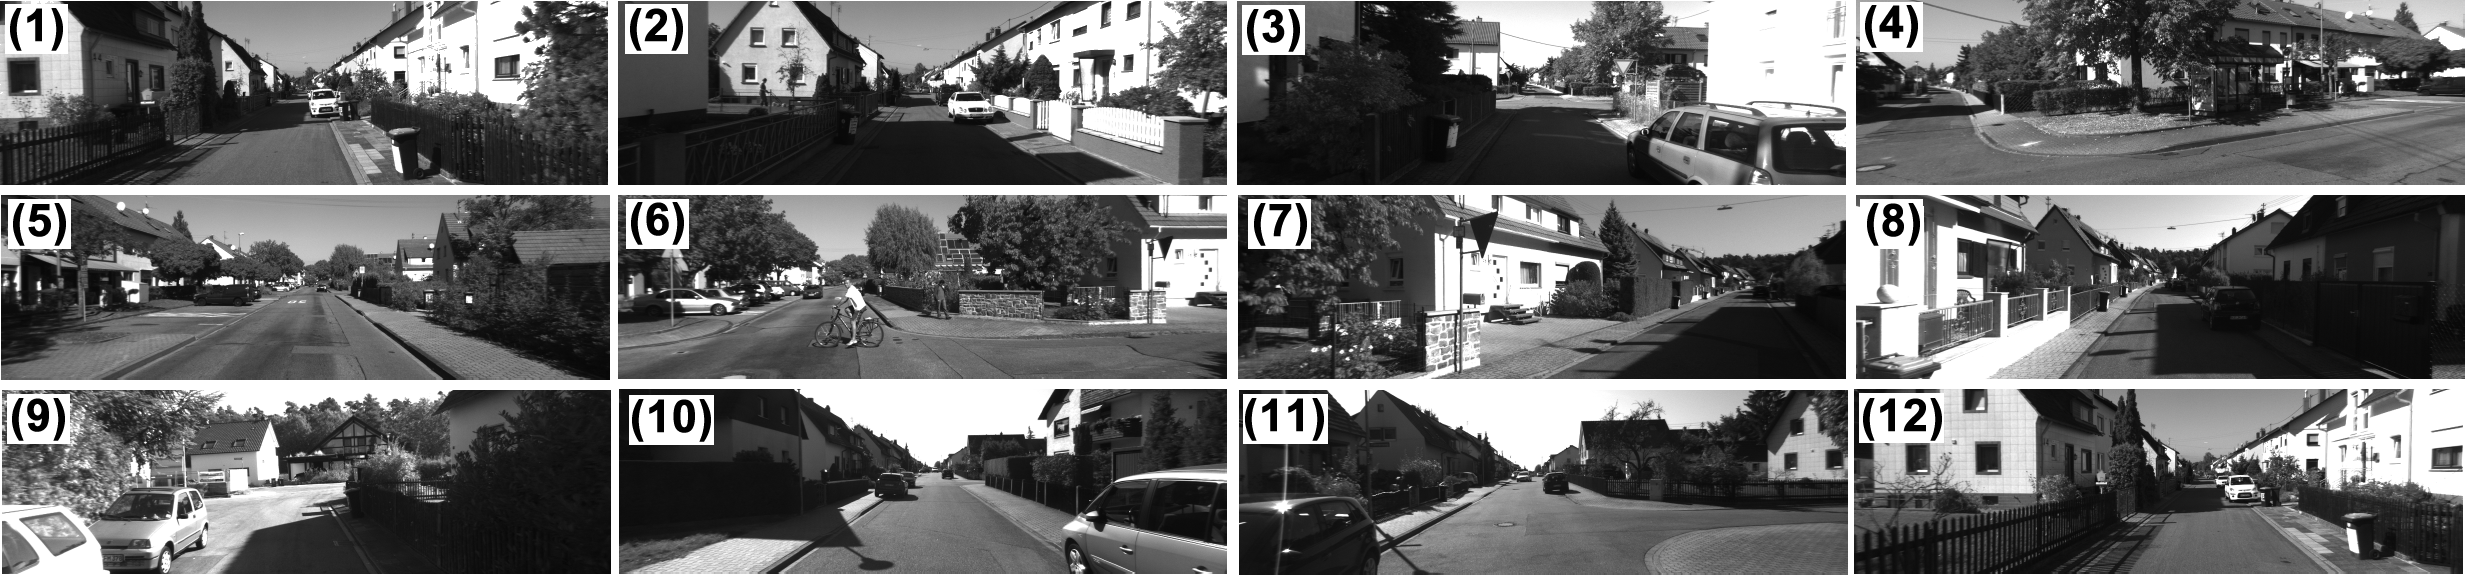
\includegraphics[width=\linewidth]{./Figures/Fig_3a.png} \\
(a) \\[0.1cm]
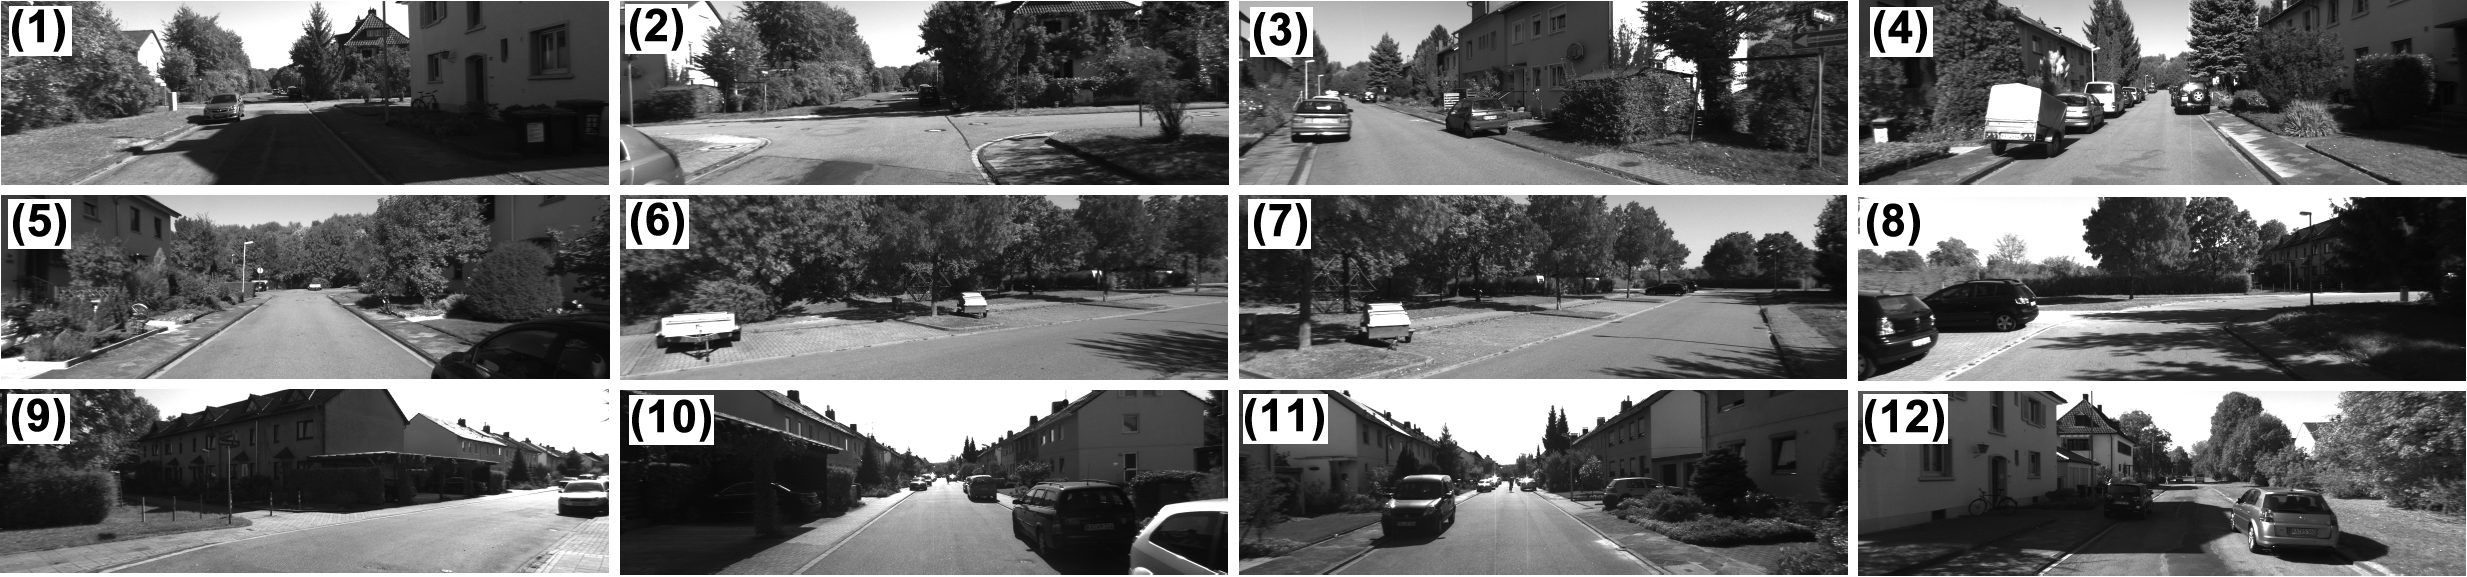
\includegraphics[width=\linewidth]{./Figures/Fig_7a.png} \\
(b)\\[0.1cm]
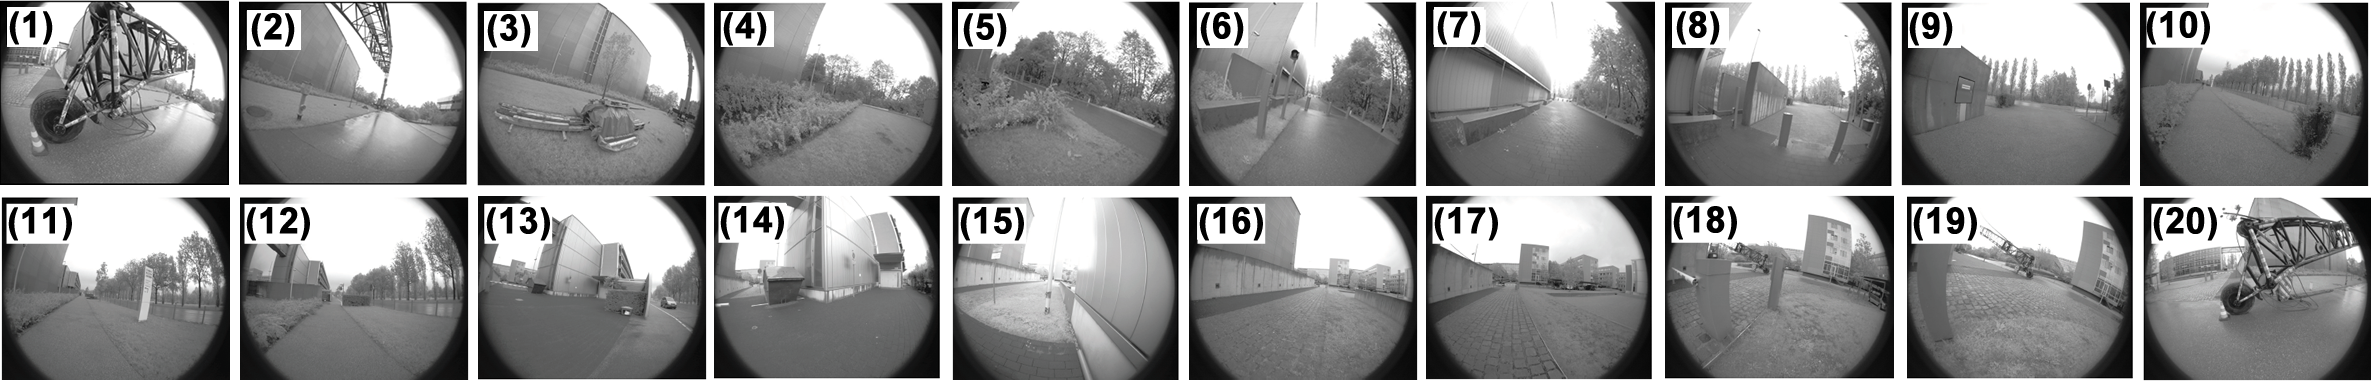
\includegraphics[width=\linewidth]{./Figures/Fig_9a.png} \\
(c)
\end{tabular}
\caption{Image Sequence from (a) Group 5 and (b) Group 8 of the KITTI dataset, and (c) Group 10 of the TUM Dataset.}
\label{fig:kitti_tum_seq}
\end{figure*}

\vspace{0.3cm}
\noindent
\emph{\textbf{Group 5}}
\vspace{0.3cm}

Fig. \ref{fig:kitti_map5} shows the trajectory of Group 5, which contains 2761 images acquired with a stable camera orientation, enabling evaluation under limited viewpoint variation. Loop Closure Detection occurs along the segments (a)-(b), (c)-(d), and (b)-(e). During navigation from (I) to (F), the camera remained fixed to the vehicle, resulting in limited rotational variation during image acquisition. Furthermore, the segment (a)-(b) corresponds to the image sequence (1)-(12) shown in Fig. \ref{fig:kitti_tum_seq}(a). Images (1) and (12) correspond to the same location, indicating a successful Loop Closure Detection event under stable viewpoint conditions.

\begin{figure}[t!]
    \centering
    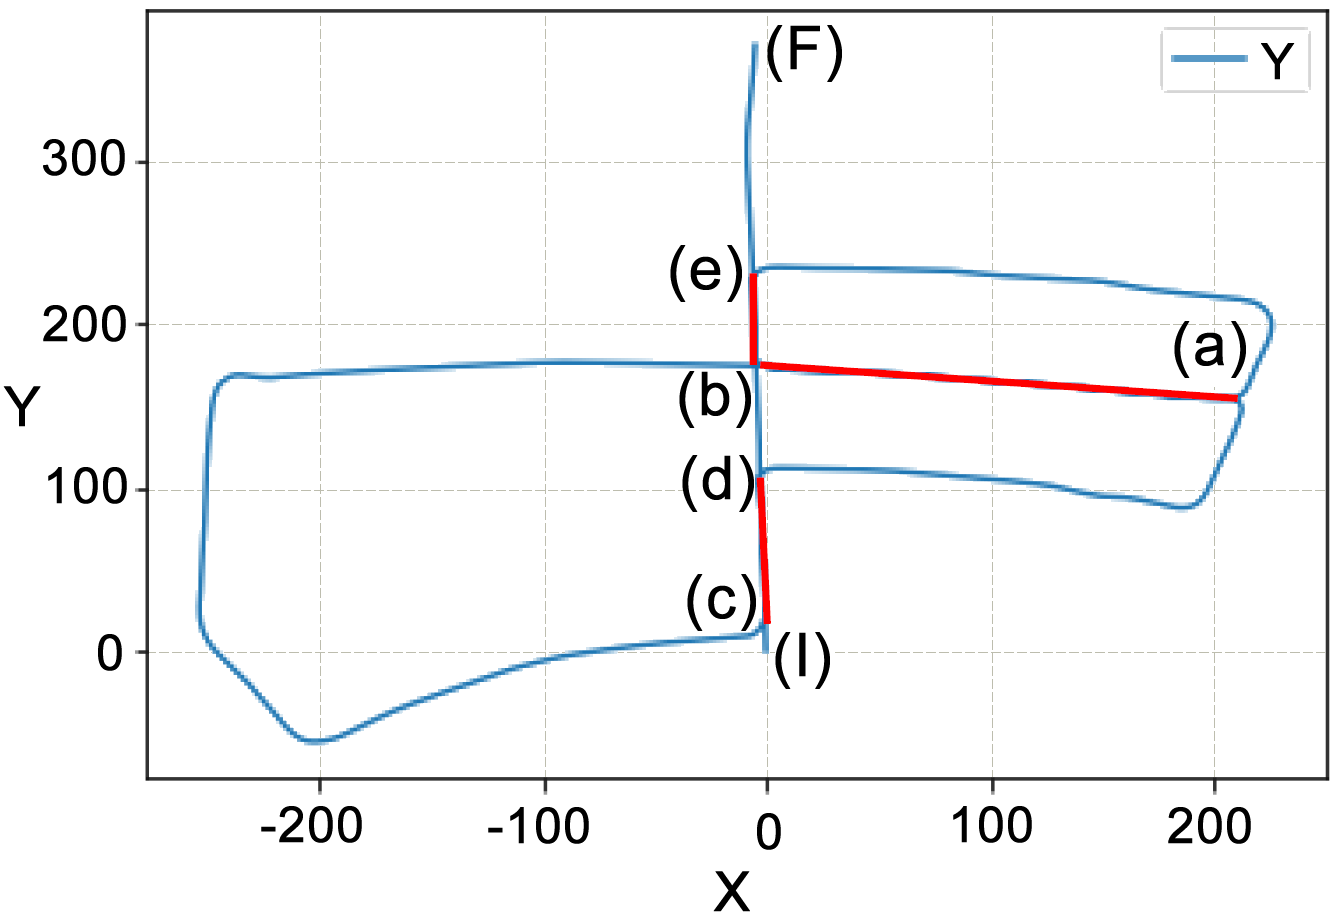
\includegraphics[width=\linewidth]{./Figures/Fig_4.png}
    \caption{Map Showing the Route Generated from Group 5 of KITTI Images.}
    \label{fig:kitti_map5}
\end{figure}   

As illustrated in Fig. \ref{fig:kitti_ex_05}, the ROC curves for (a) AlexNet, (b) ConvNeXt, (c) ResNet, and (f) Vision Transformer show comparable but limited discriminative performance. According to the results in Table \ref{tab:seq_loop_05}, the AUC values for these architectures (0.546, 0.514, 0.544, and 0.515, respectively) remain close to random classification despite the high accuracy values caused by class imbalance. In contrast, the (e) Adapted and Fine-Tuned VGG-16 achieved the highest AUC value (0.820), outperforming the Original VGG-16 (0.623) in the Loop Closure Detection task. The results indicate that task-specific fine-tuning improved descriptor discriminability under the evaluated conditions.

\begin{figure*}[t!]
    \centering
	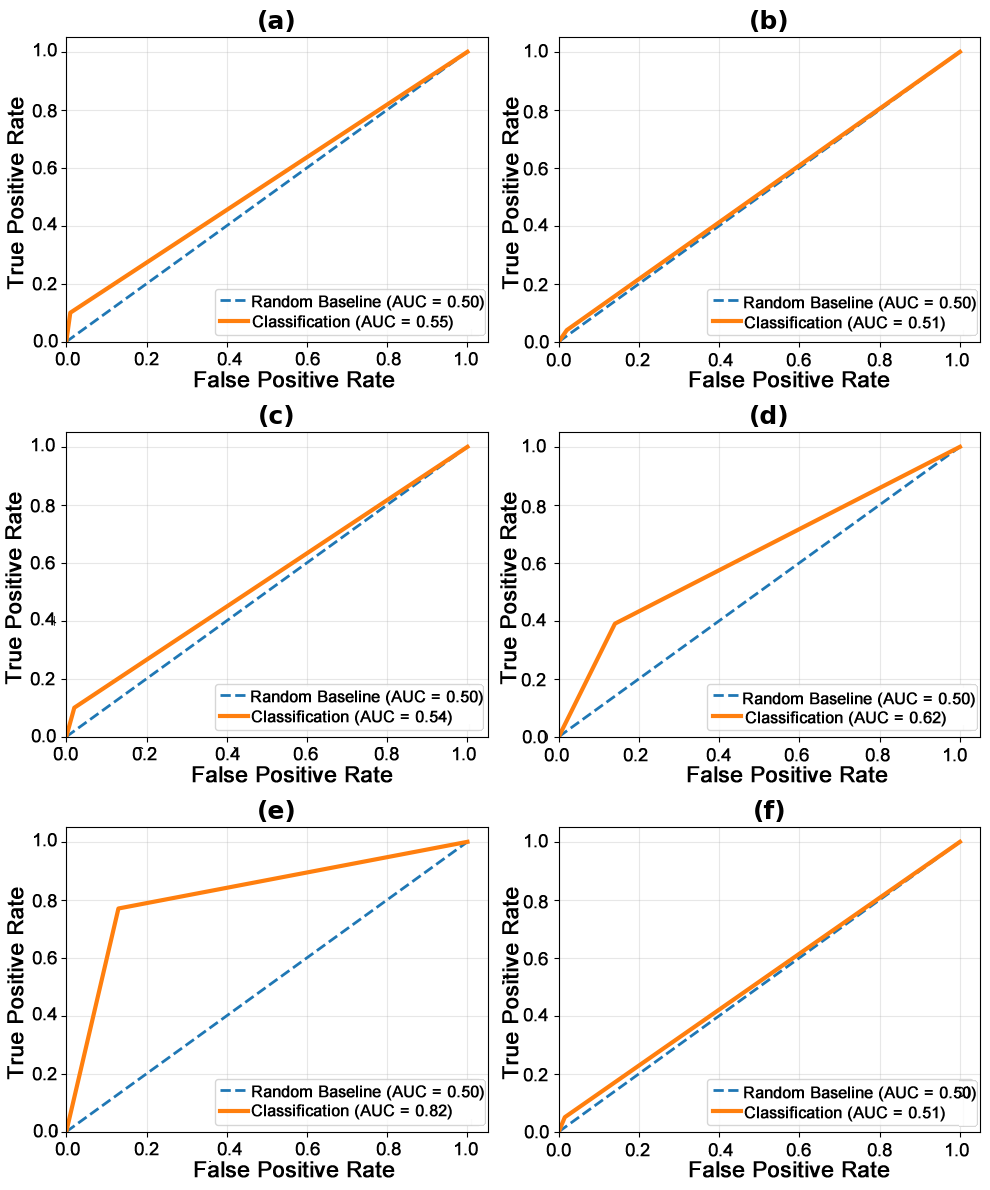
\includegraphics[width=\linewidth]{./Figures/Fig_5.png}
    \caption{KITTI Group 5 ROC Curves in (a) AlexNet, (b) ConvNeXt, (c) ResNet, (d) Original VGG-16, (e) Adapted and Fine-Tuned VGG-16, and (f) Vision Transformer.}
        \label{fig:kitti_ex_05}
\end{figure*}

Table \ref{tab:seq_loop_05} shows that the F1-score values for (a) AlexNet, (b) ConvNeXt, (c) ResNet, and (f) Vision Transformer are 0.173, 0.076, 0.171, and 0.077, respectively, all close to zero. In this case, the F1-score indicates low Precision and Sensitivity due to the low TP and high FN values in Table \ref{tab:mc_kitti05}. Accordingly, the low F1-score values indicate that these architectures failed to achieve robust Loop Closure Detection, mainly due to high FN rates.

\begin{table}[t!]
\centering
	\caption{Metrics of the Evaluated Models for Detecting Loop Closure in Group 5 of the KITTI Dataset.} 
    
\begin{tabular}{|l|c|c|c|} 
\hline
\multicolumn{1}{|c|}{\textbf{Neural Network}}                               & \textbf{Accuracy} & \textbf{F1-score} & \textbf{AUC}  \\ 
\hline
(a) AlexNet                                                              & 0.882             & 0.173                      & 0.546         \\ 
\hline
(b) ConvNeXt                                                             & 0.869             & 0.076                      & 0.514         \\ 
\hline
(c) ResNet                                                               & 0.874             & 0.171                      & 0.544         \\ 
\hline
(d) Original VGG-16                                                        & 0.802             & 0.322                      & 0.623         \\ 
\hline
\begin{tabular}[c]{@{}l@{}}(e) Adapted and Fine-\\Tuned VGG-16\end{tabular} & 0.858             & 0.570                      & 0.820         \\ 
\hline
(f) Vision Transformer                                                    & 0.870             & 0.077                      & 0.515         \\
\hline
\end{tabular}
\label{tab:seq_loop_05}
\end{table}

\begin{table}[!t]
\centering
\caption{Confusion matrix of the evaluated models.}
\label{tab:mc_kitti05}

\renewcommand{\arraystretch}{1.2}

\begin{tabular}{|c|l|c|c|c|}
\cline{4-5}

\multicolumn{3}{c|}{} &
\multicolumn{2}{c|}{\textbf{Predicted}} \\ \cline{4-5}

\multicolumn{3}{c|}{} &
\textbf{Posit.} &
\textbf{Negat.} \\ \hline

\multirow{12}{*}{\rotatebox{90}{\textbf{Actual}}}

& \multirow{2}{*}{(a) AlexNet}
& Positive & 34 & 303 \\ \cline{3-5}

& & Negative & 22 & 2402 \\ \cline{2-5}

& \multirow{2}{*}{(b) ConvNeXt}
& Positive & 15 & 322 \\ \cline{3-5}

& & Negative & 41 & 2383 \\ \cline{2-5}

& \multirow{2}{*}{(c) ResNet}
& Positive & 36 & 301 \\ \cline{3-5}

& & Negative & 47 & 2377 \\ \cline{2-5}

& \multirow{2}{*}{(d) Original VGG-16}
& Positive & 130 & 207 \\ \cline{3-5}

& & Negative & 341 & 2083 \\ \cline{2-5}

& \multirow{2}{*}{\shortstack[l]{(e) Adapted and Fine- \\Tuned VGG-16}}
& Positive & 259 & 78 \\ \cline{3-5}

& & Negative & 313 & 2111 \\ \cline{2-5}

& \multirow{2}{*}{(f) Vision Transformer}
& Positive & 15 & 322 \\ \cline{3-5}

& & Negative & 36 & 2388 \\ \hline

\end{tabular}
\end{table}

In (d) Original VGG-16, the F1-score (0.322) in Table \ref{tab:seq_loop_05} is associated with higher TP (130) and lower FN (207) shown in Table \ref{tab:mc_kitti05} compared with other DNNs. However, performance remains limited due to the high FP rate (341). In (e) Adapted and Fine-Tuned VGG-16, the higher F1-score is mainly due to increased TP (259) and reduced FN (78), although the FP value (313) remains high compared with ideal Loop Closure Detection conditions.



\subsubsection{\revinline{Descriptor-Level Reproducibility Audit}}

\begin{revisionblock}
The focused ResNet-101 audit generated 75,052 binary calibration pairs, 12,984 binary test pairs, and 8,410 binary stress pairs after excluding 3,572, 1,186, and 1,226 ambiguous pairs, respectively. Figures \ref{fig:kitti05_resnet_l1_roc} and \ref{fig:kitti05_resnet_l1_pr} compare the reconstructed legacy $L_{\infty}$ score with the corrected flattened $L_2$ score on the independent test event. Both curves were computed from continuous scores rather than binary predictions.
\end{revisionblock}

\begin{figure*}[!t]
    \centering
    \setlength{\fboxsep}{4pt}
    \colorbox{white}{\color{revisionred}%
        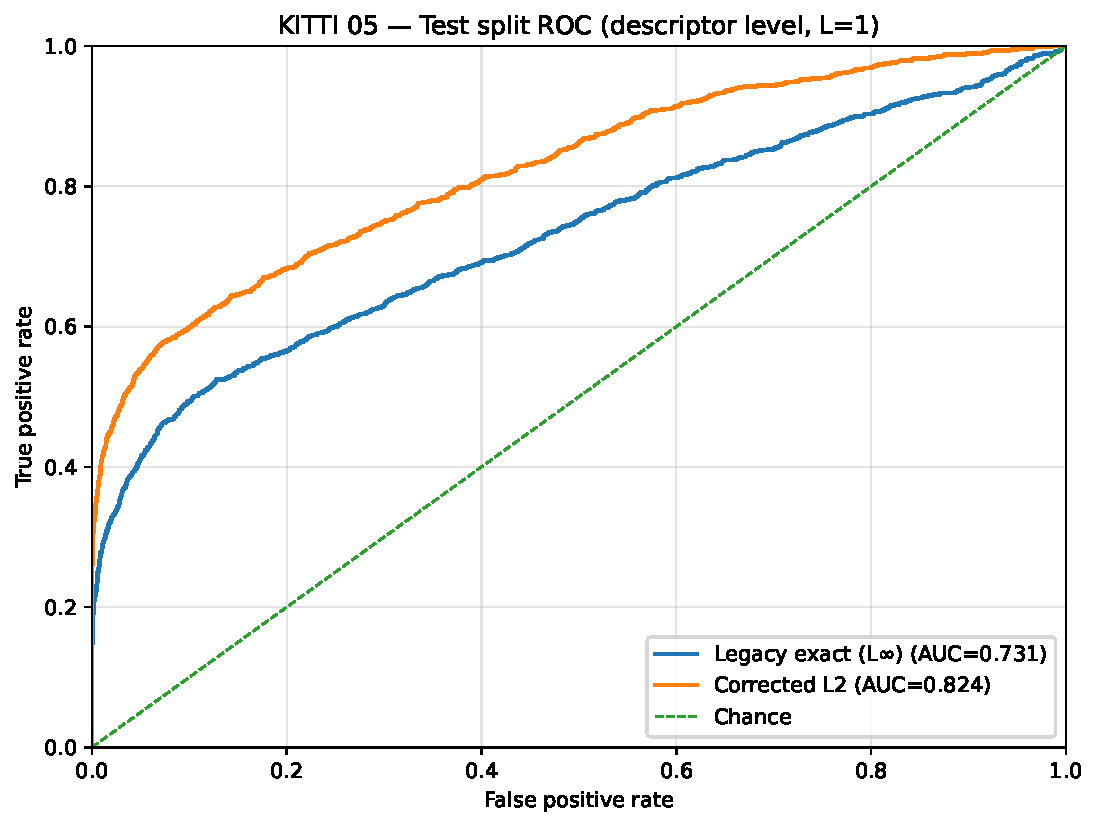
\includegraphics[
            width=\dimexpr0.86\textwidth-2\fboxsep\relax
        ]{./Figures/Fig_11_KITTI05_ResNet101_L1_ROC.pdf}%
    }
    \caption{\protect\revisioncaption{ROC curves for the reconstructed legacy $L_{\infty}$ distance and the corrected flattened $L_2$ distance on the independent KITTI 05 test event at descriptor level ($L=1$).}}
    \label{fig:kitti05_resnet_l1_roc}
\end{figure*}

\begin{figure*}[!t]
    \centering
    \setlength{\fboxsep}{4pt}
    \colorbox{white}{\color{revisionred}%
        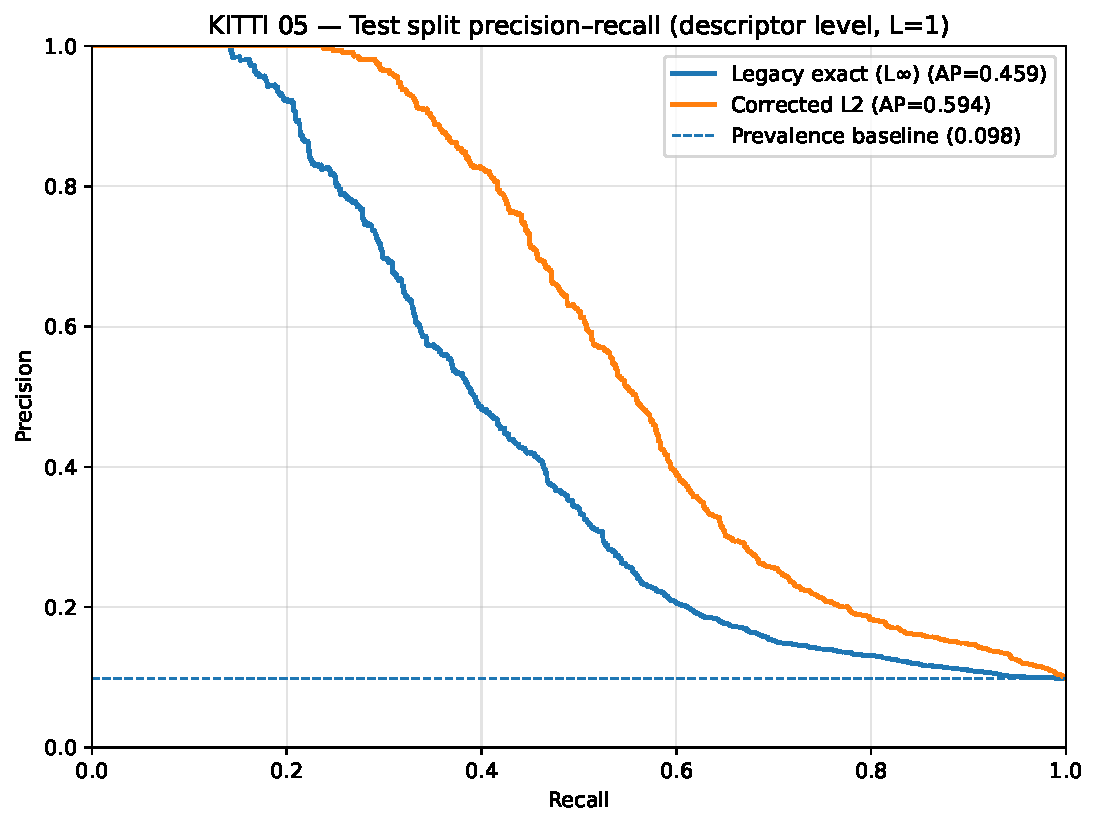
\includegraphics[
            width=\dimexpr0.86\textwidth-2\fboxsep\relax
        ]{./Figures/Fig_12_KITTI05_ResNet101_L1_PR.pdf}%
    }
    \caption{\protect\revisioncaption{Precision--recall curves for the reconstructed legacy $L_{\infty}$ distance and the corrected flattened $L_2$ distance on the independent KITTI 05 test event at descriptor level ($L=1$). The prevalence baseline emphasizes the class imbalance of the evaluation protocol.}}
    \label{fig:kitti05_resnet_l1_pr}
\end{figure*}

\begin{table*}[!t]
\centering
\caption{\protect\revisioncaption{Descriptor-level ResNet-101 results on KITTI 05. Operational F1-scores use thresholds calibrated only on the calibration event; test and stress were not recalibrated.}}
\label{tab:kitti05_resnet_l1_metrics}
\setlength{\fboxsep}{4pt}
\colorbox{white}{\color{revisionred}%
\resizebox{0.98\textwidth}{!}{%
\begin{tabular}{|l|l|c|c|c|c|}
\hline
\textbf{Split} &
\textbf{Distance} &
\textbf{ROC-AUC} &
\textbf{PR-AUC} &
\textbf{AP} &
\textbf{F1-score} \\
\hline
Calibration & Legacy $L_{\infty}$ & 0.790 & 0.419 & 0.419 & 0.422 \\
\hline
Calibration & Corrected $L_2$ & 0.785 & 0.544 & 0.544 & 0.542 \\
\hline
Test & Legacy $L_{\infty}$ & 0.731 & 0.459 & 0.459 & 0.431 \\
\hline
Test & Corrected $L_2$ & 0.824 & 0.594 & 0.594 & 0.491 \\
\hline
Stress & Legacy $L_{\infty}$ & 0.593 & 0.357 & 0.357 & 0.299 \\
\hline
Stress & Corrected $L_2$ & 0.608 & 0.393 & 0.393 & 0.337 \\
\hline
\end{tabular}%
}%
}
\end{table*}

% BEGIN REVISION: TEMPORAL ABLATION L1235
\subsubsection{\revinline{Temporal-Window Ablation}}
\label{sec:kitti05_temporal_ablation}

\begin{revisionblock}
\small
To separate descriptor discrimination from temporal verification, we evaluated one query descriptor against strict windows of $L\in\{1,2,3,5\}$ consecutive reference frames. The continuous window score is the minimum constituent similarity score, equivalently the negative maximum constituent distance. A window is positive only when all $L$ geometric pairs are positive; windows containing any ambiguous pair are excluded from binary metrics. A distinct threshold is calibrated for each method and each $L$ exclusively on the calibration event and is then frozen for the held-out test and stress events.
\end{revisionblock}

\begin{table}[!t]
\centering
\caption{\protect\revisioncaption{Temporal-window ablation on the held-out KITTI 05 test event. Metrics are reported separately for the legacy and corrected descriptor distances.}}
\label{tab:kitti05_resnet_temporal_ablation}
{\color{revisionred}
\footnotesize
\setlength{\tabcolsep}{2.4pt}
\renewcommand{\arraystretch}{0.90}
\begin{tabular}{c l c c c}
\hline
$L$ & Method & ROC-AUC & AP & F1 \\
\hline
1 & Legacy $L_\infty$ & 0.731 & 0.459 & 0.431 \\
1 & Corrected $L_2$ & 0.824 & 0.594 & 0.491 \\
\hline
2 & Legacy $L_\infty$ & 0.722 & 0.436 & 0.432 \\
2 & Corrected $L_2$ & 0.825 & 0.587 & 0.490 \\
\hline
3 & Legacy $L_\infty$ & 0.714 & 0.414 & 0.419 \\
3 & Corrected $L_2$ & 0.823 & 0.577 & 0.473 \\
\hline
5 & Legacy $L_\infty$ & 0.697 & 0.365 & 0.370 \\
5 & Corrected $L_2$ & 0.817 & 0.531 & 0.441 \\
\hline
\end{tabular}
}
\end{table}

\begin{figure}[!t]
\centering
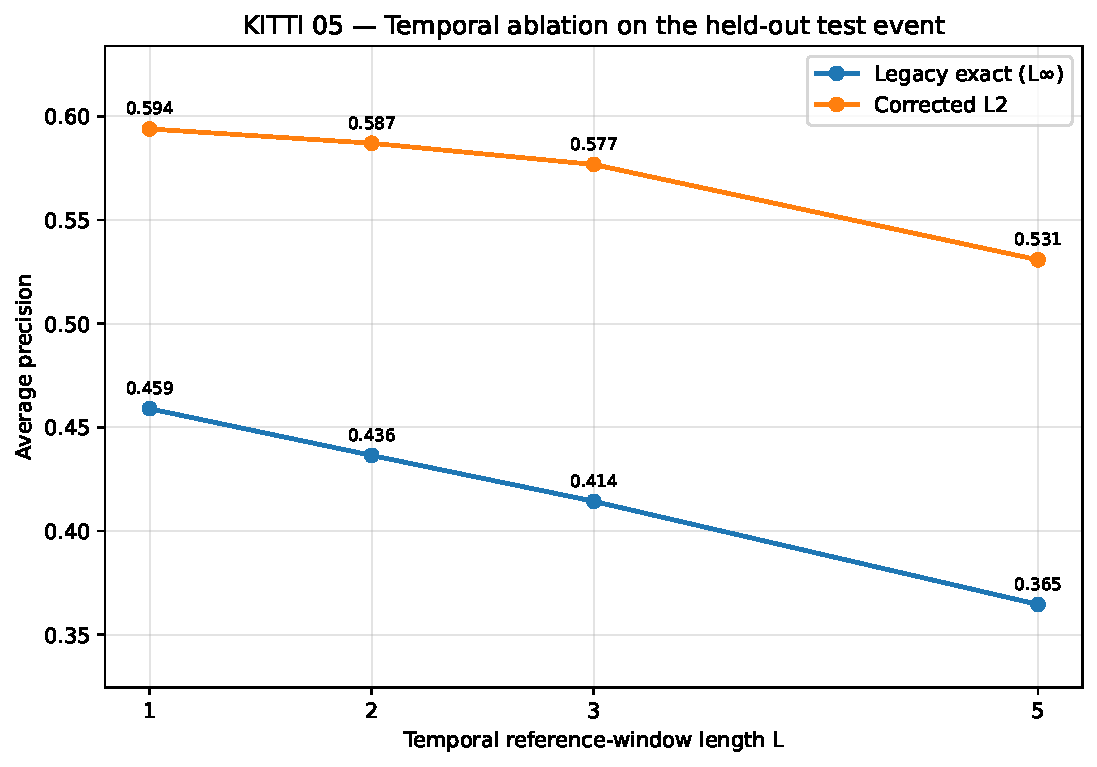
\includegraphics[
    width=0.78\columnwidth
]{./Figures/Fig_13_KITTI05_ResNet101_Temporal_AP.pdf}
\caption{\protect\revisioncaption{Test AP versus temporal window length $L$ on KITTI 05.}}
\label{fig:kitti05_resnet_temporal_ap}
\end{figure}

\begin{figure}[!t]
\centering
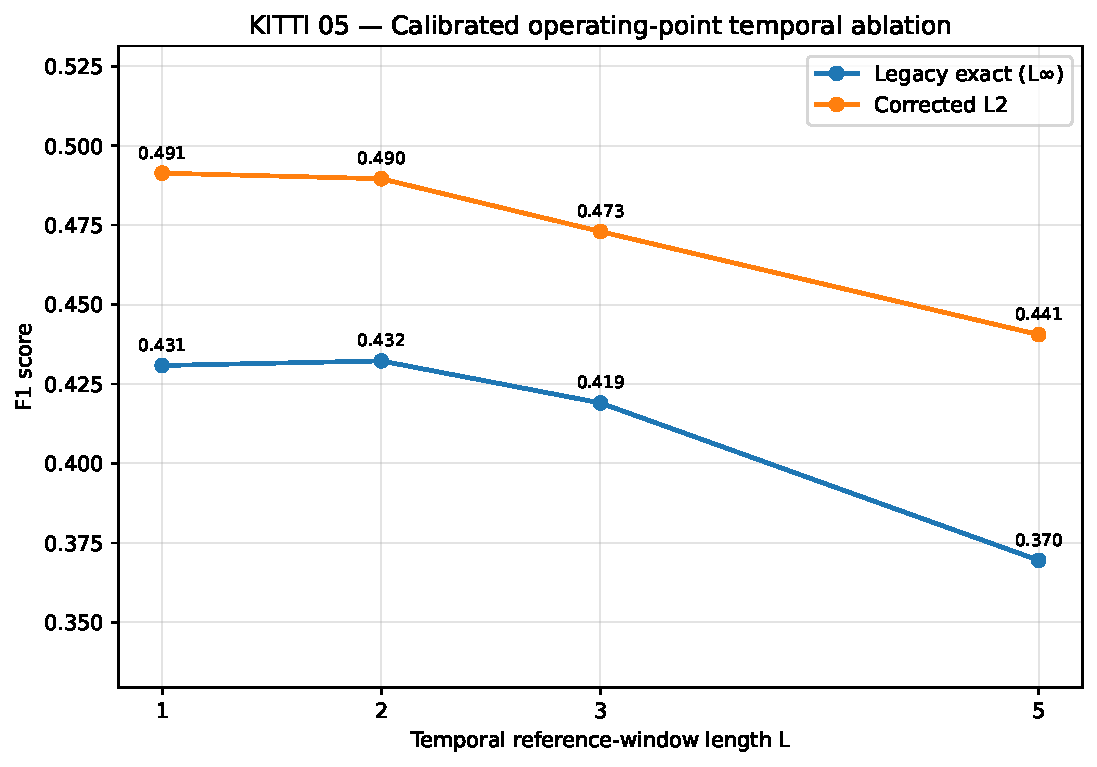
\includegraphics[
    width=0.78\columnwidth
]{./Figures/Fig_14_KITTI05_ResNet101_Temporal_F1.pdf}
\caption{\protect\revisioncaption{Test F1 versus temporal window length $L$ on KITTI 05.}}
\label{fig:kitti05_resnet_temporal_f1}
\end{figure}

\begin{revisionblock}
\small
The corrected descriptor achieved its highest test ROC-AUC at $L=2$ (0.824784), but the increase over $L=1$ was only +0.000286. In contrast, AP changed from 0.593918 at $L=1$ to 0.587019 at $L=2$ (-0.006899), while F1 changed from 0.491369 to 0.489590 (-0.001779). Longer strict windows degraded both ranking and operating-point performance: at $L=5$, AP and F1 decreased by -0.063165 and -0.050841, respectively, relative to $L=1$. Therefore, the original three-match rule is not treated as an intrinsic property of the descriptor. Descriptor-level performance is reported at $L=1$, and temporal verification is reported separately as an ablation.
\end{revisionblock}
% END REVISION: TEMPORAL ABLATION L1235


\begin{revisionblock}
As summarized in Table \ref{tab:kitti05_resnet_l1_metrics}, the corrected $L_2$ formulation achieved the strongest transfer to the independent test event, increasing ROC-AUC from $0.731$ to $0.824$, AP from $0.459$ to $0.594$, and F1-score from $0.431$ to $0.491$ relative to the reconstructed legacy formulation. On the stress event, the corrected formulation also improved ROC-AUC from $0.593$ to $0.608$, AP from $0.357$ to $0.393$, and F1-score from $0.299$ to $0.337$. Although the legacy formulation produced a slightly higher calibration ROC-AUC ($0.790$ versus $0.785$), the corrected formulation yielded substantially higher calibration AP ($0.544$ versus $0.419$) and F1-score ($0.542$ versus $0.422$). The calibration-derived distance thresholds were $2.704$ for the legacy $L_{\infty}$ formulation and $21.822$ for the corrected $L_2$ formulation. Because the test and stress thresholds were fixed before evaluation, their F1-scores measure operating-point transfer rather than split-specific threshold optimization.
\end{revisionblock}

\vspace{0.3cm}
\noindent
\emph{\textbf{Group 8}}
\vspace{0.3cm}

Group 8 of the KITTI dataset comprises 4071 images tracing the trajectory illustrated in Fig. \ref{fig:kitti_map8}, originating at point (I) and finishing at (F). The sequence (1)-(12) presented in Fig. \ref{fig:kitti_tum_seq}(b) corresponds to the path segment (d)-(c) in Fig. \ref{fig:kitti_map8}. Notably, images (1) and (12) were captured at the same spatial location but from opposing headings. Within Group 8, two distinct paths are identified: (a)-(b) and (c)-(d). Loop Closure Detection occurs when these segments are revisited from the opposite traversal directions; specifically, the initial traversals from (a) to (b) and (c) to (d) are subsequently revisited along the trajectories (d) to (c) and (b) to (a).  

\begin{figure}[t!]
    \centering
    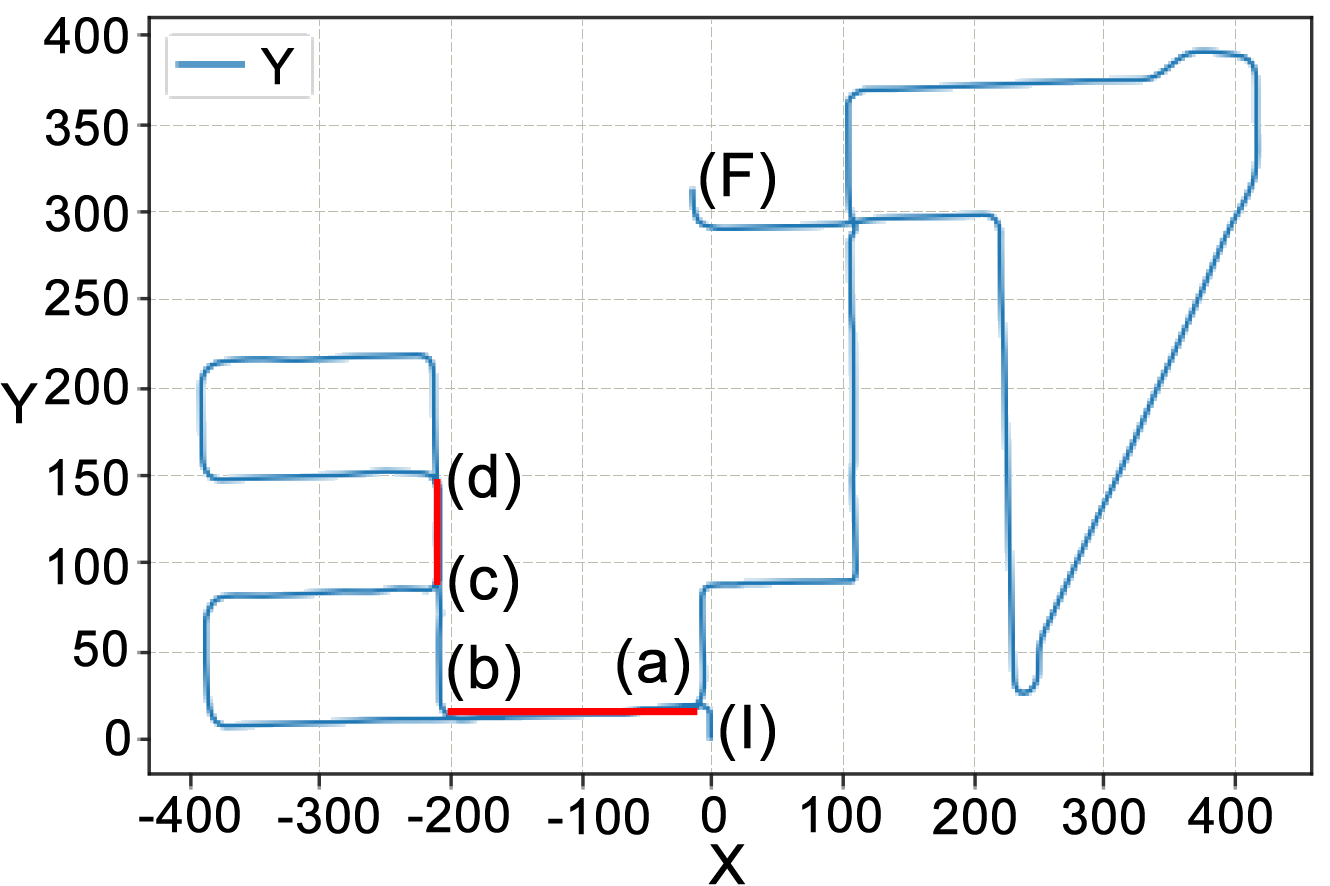
\includegraphics[width=\linewidth]{./Figures/Fig_6.png}
    \caption{Path Generated from Images in Group 8 of the KITTI Dataset.}  
    \label{fig:kitti_map8}
\end{figure}   

As shown in Table \ref{tab:seq_loop_08}, (a) AlexNet, (b) ConvNeXt, (d) Original VGG-16, and (f) Vision Transformer exhibited the lowest Loop Closure Detection performance. The ROC curves for (a) AlexNet and (d) Original VGG-16 are shown in Figs. \ref{fig:kitti_ex_08}(a) and \ref{fig:kitti_ex_08}(c), respectively, whereas (b) ConvNeXt and (f) Vision Transformer are represented by the ROC curve in Fig. \ref{fig:kitti_y}. Because the AUC values of (b) ConvNeXt and (f) Vision Transformer are close to 0.50, both architectures exhibit near-random classification behavior, indicating limited discriminative capability for Loop Closure Detection under opposite traversal conditions.

\begin{table}[t!]
    \centering
    \caption{Metrics of the Evaluated Models for Detecting Loop Closure in Group 8 of the KITTI Dataset.}
    \begin{tabular}{|l|c|c|c|} 
    \hline
    \multicolumn{1}{|c|}{\textbf{DNN}}                               & \textbf{Accuracy} & \textbf{F1-\textit{Score}} & \textbf{AUC}  \\ 
    \hline
    (a) AlexNet                                                              & 0.920             & 0.198                      & 0.556         \\ 
    \hline
    (b) ConvNeXt                                                             & 0.867             & 0.078                      & 0.504         \\ 
    \hline
    (c) ResNet                                                               & 0.887             & 0.454                      & 0.751         \\ 
    \hline
    (d) Original VGG-16                                                      & 0.914             & 0.273                      & 0.589         \\ 
    \hline
    \begin{tabular}[c]{@{}l@{}}(e) Adapted and Fine-\\Tuned VGG-16\end{tabular} & 0.902             & 0.361                      & 0.648         \\ 
    \hline
    (f) Vision Transformer                                                     & 0.900             & 0.005                      & 0.495         \\
    \hline
\end{tabular}
\label{tab:seq_loop_08}
\end{table}

\begin{figure*}[t!]
    \centering
	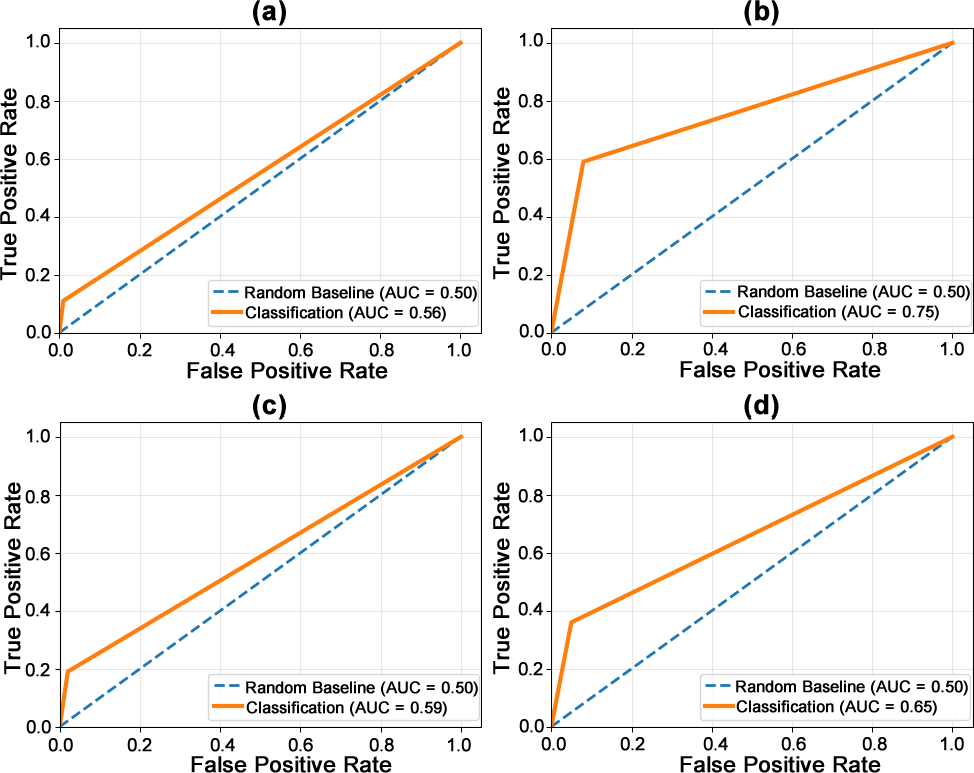
\includegraphics[width=\linewidth]{./Figures/Fig_8x.png}
    \caption{ROC Curves for KITTI Group 8 in (a) AlexNet, (b) ResNet, (c) Original VGG-16, and (d) Adapted and Fine-Tuned VGG-16.}
    \label{fig:kitti_ex_08}
\end{figure*}

\begin{figure}[t!]
    \centering
    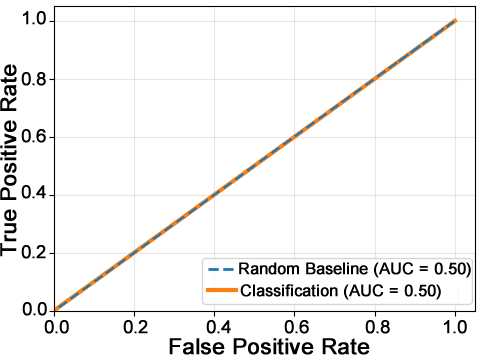
\includegraphics[width=\linewidth]{./Figures/Fig_8y.png}
    \caption{Representative ROC Curve for Architectures Exhibiting Near-Random Classification Performance (AUC $\approx 0.50$).}  
    \label{fig:kitti_y}
\end{figure}  

In Group 8, the Accuracies for detecting Loop Closure were high, as shown in Table  \ref{tab:seq_loop_08}. However, F1-scores near zero indicate low Precision and Sensitivity, showing that Accuracy alone was insufficient to evaluate performance. Additionally, an AUC close to 0.500 indicates that the detection was ineffective.

The F1-score in Table \ref{tab:seq_loop_08} indicates that (c) ResNet achieved the best result (0.454) due to the high TP (191) and relatively low FN (133) shown in Table \ref{tab:mc_kitti08}. However, the architecture also produced a high FP value (326) compared with the other evaluated models, reducing Precision despite the improved Recall. Nevertheless, the results demonstrate that (c) ResNet had the best trade-off among the evaluated architectures between detection capability and robustness in detecting Loop Closure, despite the increased FP rate. 

\begin{table}[!t]
\centering
\caption{Confusion Matrix of DNN for Detecting Loop Closure in Group 8 of KITTI.}
\label{tab:mc_kitti08}

\renewcommand{\arraystretch}{1.2}

\begin{tabular}{|c|l|c|c|c|}
\cline{4-5}

\multicolumn{3}{c|}{} &
\multicolumn{2}{c|}{\textbf{Predicted}} \\ \cline{4-5}

\multicolumn{3}{c|}{} &
\textbf{Posit.} &
\textbf{Negat.} \\ \hline

\multirow{12}{*}{\rotatebox{90}{\textbf{Actual}}}

& \multirow{2}{*}{(a) AlexNet}
& Positive & 40 & 284 \\ \cline{3-5}

& & Negative & 41 & 3705 \\ \cline{2-5}

& \multirow{2}{*}{(b) ConvNeXt}
& Positive & 23 & 301 \\ \cline{3-5}

& & Negative & 239 & 3507 \\ \cline{2-5}

& \multirow{2}{*}{(c) ResNet}
& Positive & 191 & 133 \\ \cline{3-5}

& & Negative & 326 & 3420 \\ \cline{2-5}

& \multirow{2}{*}{(d) Original VGG-16}
& Positive & 65 & 259 \\ \cline{3-5}

& & Negative & 88 & 3658 \\ \cline{2-5}

& \multirow{2}{*}{\shortstack[l]{(e) Adapted and Fine-\\Tuned VGG-16}}
& Positive & 112 & 212 \\ \cline{3-5}

& & Negative & 185 & 3561 \\ \cline{2-5}

& \multirow{2}{*}{(f) Vision Transformer}
& Positive & 1 & 323 \\ \cline{3-5}

& & Negative & 47 & 3699 \\ \hline

\end{tabular}
\end{table}

In (e) Adapted and Fine-Tuned VGG-16, the F1-score of 0.361 in Table \ref{tab:seq_loop_08} indicates limited Precision and Recall, primarily because the FN (212) and FP (185) values are relatively high compared with the TP value (112) shown in Table \ref{tab:mc_kitti08}. In this case, Loop Closure Detection was identified, but its performance was worse than in (c) ResNet due to the lower TP value.

In Group 5, the Adapted and Fine-Tuned VGG-16 achieved the best results for Loop Closure Detection, demonstrating the best performance in real-world outdoor environments. In Group 8, ResNet performed the best. In this group, it was found that the opposite direction affected the performance in detecting Loop Closure. These results suggest that opposite traversal directions affect descriptor consistency, particularly for architectures not explicitly optimized for viewpoint invariance.

\subsection{TUM}

The research group at the Technical University of Munich (TUM) provides datasets for Computer Vision, Image Processing, and Pattern Recognition. One of these datasets is Monocular Visual Odometry, which contains 50 groups of sequential images captured in various real-world indoor and outdoor environments. The dataset also includes monocular image sequences under varying camera motion and rotational conditions. 

To evaluate the Loop Closure Detection described in Section \ref{sec:Loop}, Group 19 of the TUM dataset was used, as it exhibits Loop Closure and contains images of outdoor environments. The group consists of 8300 images captured by a monocular camera with varying camera orientations. The sequences (1)-(20) in Fig. \ref{fig:kitti_tum_seq}(c) illustrate the path used to detect Loop Closure, which occurs in image (20) during the return to the starting point (1). 

Table \ref{tab:seq_loop_tum} shows that (a) AlexNet, (b) ConvNeXt, (d) Original VGG-16, and (f) Vision Transformer achieved AUC values close to 0.50, reflecting near-random classification performance and limited capability for Loop Closure Detection. Consequently, their accuracy values should not be interpreted in isolation. The representative ROC curve presented in Fig. \ref{fig:kitti_y} illustrates the near-random classification behavior observed for these architectures. In contrast, Fig. \ref{fig:tum_ex} highlights that (c) ResNet and (e) Adapted and Fine-Tuned VGG-16 achieved AUC values of 0.644 and 0.662, respectively, demonstrating superior discrimination between positive and negative Loop Closure samples.


\begin{figure*}[t!]
    \centering
	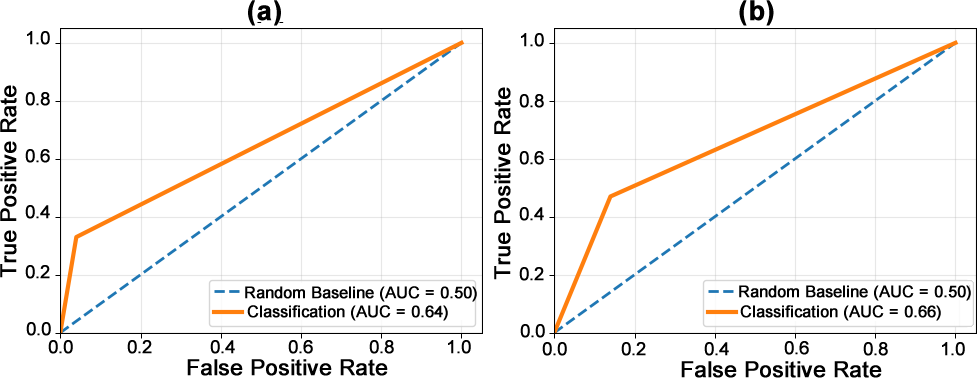
\includegraphics[width=\linewidth]{./Figures/Fig_10x.png}
    \caption{ROC Curves for ResNet and Adapted and Fine-Tuned VGG-16 on TUM Group 19.}
    \label{fig:tum_ex}
\end{figure*}

The F1-scores in Table \ref{tab:seq_loop_tum} indicate low Precision and Recall for (a) AlexNet (0.045), (b) ConvNeXt (0.046), (d) Original VGG-16 (0.048), and (f) Vision Transformer (0.043). This is due to low TP values, which range from 23 to 24, as shown in Table \ref{tab:mc_tum}. In these cases, the results indicate poor performance in detecting Loop Closure. 

\begin{table}[t!]
\centering
\caption{DNN Metrics for Detecting Loop Closure in TUM Group 19.}
\begin{tabular}{|l|c|c|c|} 
\hline
\multicolumn{1}{|c|}{\textbf{DNN}}                               & \textbf{Accuracy} & \textbf{F1-\textit{Score}} & \textbf{AUC}  \\ 
\hline
(a) AlexNet                                                              & 0.883             & 0.045                      & 0.498         \\ 
\hline
(b) ConvNeXt                                                             & 0.885             & 0.046                      & 0.499         \\ 
\hline
(c) ResNet                                                               & 0.908             & 0.382                      & 0.644         \\ 
\hline
(d) Original VGG-16                                                      & 0.887             & 0.048                      & 0.500         \\ 
\hline
\begin{tabular}[c]{@{}l@{}}(e) Adapted and Fine-\\Tuned VGG-16 \end{tabular} & 0.828             & 0.317                      & 0.662         \\ 
\hline
(f) Vision Transformer                                                    & 0.838             & 0.043                      & 0.459         \\
\hline
\end{tabular}
\label{tab:seq_loop_tum}
\end{table}

The (e) Adapted and Fine-Tuned VGG-16 achieved a relatively high TP (185) but also a high FN (389) in Table \ref{tab:mc_tum}, resulting in an F1-score of 0.317, as shown in Table \ref{tab:seq_loop_tum}. This indicates that Loop Closure Detection was identified, though with low Precision. However, the (c) ResNet achieved a higher TP of 234 and an F1-score of 0.382, reflecting a moderate improvement in descriptor matching reliability and overall better performance in detecting Loop Closure.

\begin{table}[!t]
    \centering
    \caption{Confusion Matrices of the Evaluated Models for Detecting Loop Closure in Group 19 of the TUM Dataset.}
    \label{tab:mc_tum}

    \renewcommand{\arraystretch}{1.2}
    \begin{tabular}{|c|l|c|c|c|}
    \cline{4-5}
    \multicolumn{3}{c|}{} &
    \multicolumn{2}{c|}{\textbf{Predicted}} \\ \cline{4-5}

    \multicolumn{3}{c|}{} &
    \textbf{Posit.} &
    \textbf{Negat.} \\ \hline

    \multirow{12}{*}{\rotatebox{90}{\textbf{Actual}}}
    & \multirow{2}{*}{(a) AlexNet}
    & Positive & 23 & 698 \\ \cline{3-5}
    & & Negative & 275 & 7304 \\ \cline{2-5}
    & \multirow{2}{*}{(b) ConvNeXt} 
    & Positive & 23 & 699 \\ \cline{3-5}
    & & Negative & 273 & 7305 \\ \cline{2-5}
    & \multirow{2}{*}{(c) ResNet}
    & Positive & 234 & 487 \\ \cline{3-5}
    & & Negative & 271 & 7308 \\ \cline{2-5}
    & \multirow{2}{*}{(d) Original VGG-16}
    & Positive & 24 & 697 \\ \cline{3-5}
    & & Negative & 1040 & 6394 \\ \cline{2-5}
    & \multirow{2}{*}{\shortstack[l]{(e) Adapted and Fine-\\Tuned VGG-16}}
    & Positive & 185 & 389 \\ \cline{3-5}
    & & Negative & 240 & 7539 \\ \cline{2-5}
    & \multirow{2}{*}{(f) Vision Transformer}
    & Positive & 23 & 721 \\ \cline{3-5}
    & & Negative & 621 & 6935 \\ \hline
\end{tabular}
\end{table}

The Adapted and Fine-Tuned VGG-16 achieved improved Loop Closure Detection performance on the TUM dataset. Nevertheless, significant camera rotations during image acquisition substantially degraded descriptor consistency, increasing FP and FN rates during image matching. These effects reduced descriptor discriminability, resulting in lower AUC and F1-score values, as summarized in Tables \ref{tab:mc_tum} and \ref{tab:seq_loop_tum}.

\subsection{Comparative Discussions}

The experimental results indicate that descriptor performance varies across operational conditions and representation learning strategies. The Adapted and Fine-Tuned VGG-16 achieved superior performance under stable viewpoint conditions, suggesting that task-specific fine-tuning improved descriptor discriminability for Loop Closure Detection. In contrast, ResNet demonstrated greater robustness under opposite traversal conditions, possibly benefiting from the improved feature generalization enabled by residual learning.

The Transformer-based architecture showed limited robustness across the evaluated scenarios. One possible explanation is that the pretrained Vision Transformer was not specifically optimized for Visual Place Recognition tasks, resulting in descriptor representations that are less invariant to viewpoint and appearance changes.

The experiments also revealed that opposite traversal directions and camera rotations significantly increased FP and FN rates during descriptor matching. These operational conditions continue to represent challenges for Loop Closure Detection in Visual SLAM, particularly in large-scale environments.

Overall, the results indicate that descriptor suitability for Visual SLAM depends not only on feature representation capacity but also on operational robustness under viewpoint variations, traversal direction changes, and camera rotation.

Because ROC analysis evaluates descriptor discrimination across multiple decision thresholds, the AUC values reported in this work provide a threshold-independent assessment of descriptor robustness under viewpoint variation, opposite traversal directions, and camera rotation conditions.

\begin{revisionblock}
The descriptor-level audit further demonstrates why precision--recall analysis is necessary for Loop Closure Detection. On the independent test event, the positive prevalence was approximately $0.098$, and ROC-AUC alone did not fully express the difference between the distance formulations. The corrected $L_2$ score achieved AP $=0.594$, compared with AP $=0.459$ for the reconstructed legacy score, while also reducing false positives at the fixed calibration-derived threshold. Nevertheless, both formulations degraded on the stress event, indicating that descriptor-distance correction improves the reproducibility and discrimination of the pipeline but does not eliminate the difficulty of challenging revisit conditions. These focused audit values should not be numerically merged with the historical multi-architecture results in Tables \ref{tab:seq_loop_05}, \ref{tab:seq_loop_08}, and \ref{tab:seq_loop_tum}, because the audit uses an explicit event-level split, a revised candidate-pair protocol, and descriptor-level $L=1$ evaluation.
\end{revisionblock}



% BEGIN KITTI05_SOTA_L1_REVISION
{\color{red}
\refstepcounter{subsection}
\subsection*{\textcolor{red}{E. Comparison with Place-Recognition Baselines}}
\label{subsec:kitti05_sota_l1}

To isolate descriptor quality from the temporal verification stage, we compared all methods at descriptor level ($L=1$) using exactly the same KITTI-05 candidate pairs, spatial labels, and data partitions. A positive pair has a spatial distance of at most $5$~m, pairs between $5$ and $10$~m are retained as ambiguous but excluded from binary metrics, and pairs at or above $10$~m are negative. For every method, the decision threshold was selected only on the calibration partition by maximizing the F1 score and was then frozen for the independent test and stress partitions. The comparison includes the original ResNet-101 score, the corrected flattened Euclidean score, the classical DBoW2 place-recognition model~\cite{GalvezLopez2012DBoW2} instantiated with the canonical ORB-SLAM2 vocabulary~\cite{MurArtal2017ORBSLAM2}, and a 512-dimensional NetVLAD descriptor~\cite{Arandjelovic2016NetVLAD}.

\begin{table}[H]
\centering
\color{red}
\captionsetup{labelfont={color=red},textfont={color=red}}
\caption{\color{red}Descriptor-level loop-closure performance on the KITTI-05 test partition. Thresholds were calibrated exclusively on the calibration partition; ambiguous pairs were excluded from binary metrics.}
\label{tab:kitti05_sota_l1}
\footnotesize
\setlength{\tabcolsep}{2.6pt}
\begin{tabular}{lccccc}
\toprule
Method & ROC--AUC & AP & Precision & Recall & F1 \\
\midrule
ResNet-101 (legacy) & 0.731 & 0.459 & 0.643 & 0.324 & 0.431 \\
ResNet-101 (L2) & 0.824 & 0.594 & 0.910 & 0.336 & 0.491 \\
ORB-SLAM2 DBoW2 & 0.868 & 0.764 & \textbf{0.998} & 0.336 & 0.503 \\
NetVLAD-512 & \textbf{0.904} & \textbf{0.848} & 0.958 & \textbf{0.771} & \textbf{0.854} \\
\bottomrule
\end{tabular}
\end{table}

Table~\ref{tab:kitti05_sota_l1} and Fig.~\ref{fig:kitti05_sota_l1_curves} show that NetVLAD-512 provides the strongest overall ranking and operating-point performance, reaching a test ROC--AUC of $0.904$, AP of $0.848$, and F1 of $0.854$. DBoW2 is substantially more conservative: it produces only one false positive on the test partition and therefore reaches a precision of $0.998$, but its recall is limited to $0.336$. The corrected ResNet-101 distance improves over the legacy score in ROC--AUC, AP, precision, and F1, confirming that descriptor geometry contributes independently of temporal verification. Nevertheless, both classical DBoW2 and learned NetVLAD outperform the corrected ResNet score in ROC--AUC and AP under the same calibration protocol.

\begin{figure*}[!t]
\centering
\color{red}
\captionsetup{labelfont={color=red},textfont={color=red}}
\begin{minipage}[t]{0.485\textwidth}
\centering
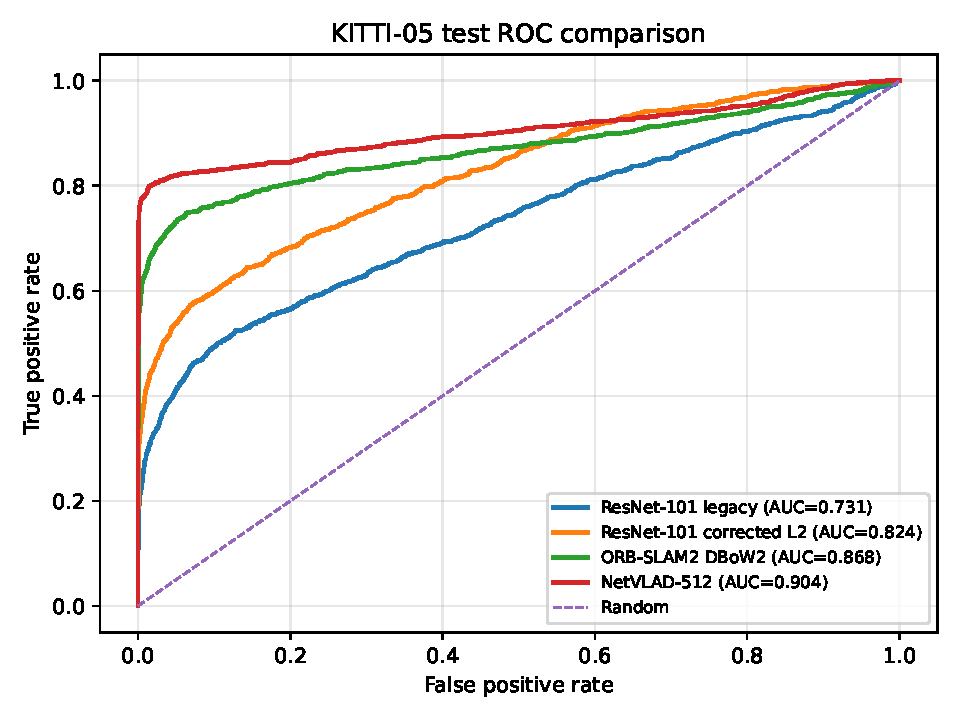
\includegraphics[width=\linewidth]{figures/kitti05_sota_l1_test_roc.pdf}
\textcolor{red}{(a) Receiver operating characteristic.}
\end{minipage}
\hfill
\begin{minipage}[t]{0.485\textwidth}
\centering
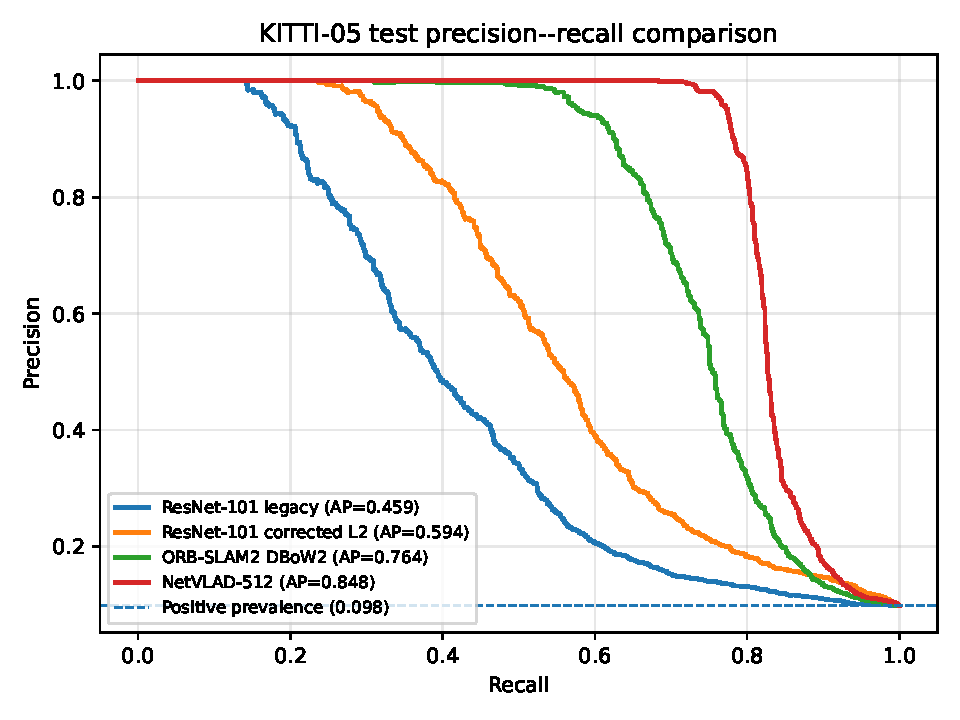
\includegraphics[width=\linewidth]{figures/kitti05_sota_l1_test_pr.pdf}
\textcolor{red}{(b) Precision--recall characteristic.}
\end{minipage}
\caption{\color{red}Descriptor-level comparison on the KITTI-05 test partition using continuous similarity scores. The ROC curves summarize ranking across false-positive rates, whereas the precision--recall curves emphasize performance under the imbalanced positive/negative distribution.}
\label{fig:kitti05_sota_l1_curves}
\end{figure*}
}
% END KITTI05_SOTA_L1_REVISION

% BEGIN KITTI05_EFFICIENCY_REVISION
{\color{red}
\refstepcounter{subsection}
\subsection*{\textcolor{red}{F. Implementation-Level Efficiency}}
\label{subsec:kitti05_efficiency}

To complement the descriptor-level accuracy analysis, we measured extraction latency, exhaustive comparison latency, descriptor storage, and memory consumption for the three implementations used in the KITTI-05 baseline study. Each benchmark used a batch size of one, 20 warm-up executions, three rounds of 100 measured images, and excluded image-file reading from the timed region. ResNet-101 was executed on the CPU with four threads, ORB-SLAM2 DBoW2 on one CPU thread, and NetVLAD-512 on an NVIDIA GeForce MX150 GPU. For NetVLAD, the decomposed and complete-pipeline measurements were interleaved with a balanced order to reduce clock and thermal drift. Consequently, Table~\ref{tab:kitti05_efficiency} characterizes the evaluated implementations on the stated hardware; it must not be interpreted as a hardware-independent ranking of architectural complexity.

\begin{table*}[!t]
\color{red}
\captionsetup{labelfont={color=red},textfont={color=red}}
\caption{\textcolor{red}{Controlled KITTI-05 implementation-level efficiency. Extraction reports the mean end-to-end descriptor latency, while matching reports exhaustive scoring against 2,761 stored descriptors. Device and thread differences are shown explicitly.}}
\label{tab:kitti05_efficiency}
\centering
\scriptsize
\setlength{\tabcolsep}{3.2pt}
\begin{tabular}{l l r r r r r r}
\toprule
Method & Extraction device & Ext. (ms) & FPS & Dim. & Storage (KiB) & Match (ms) & RSS (MiB) \\
\midrule
ResNet-101 ($L_2$) &
CPU, 4 threads &
189.08 &
5.29 &
4096 &
16.00 &
23.38 &
1495.5 \\
ORB-SLAM2 DBoW2 &
CPU, 1 thread &
13.03 &
76.72 &
sparse BoW &
11.41 &
155.75 &
676.7 \\
NetVLAD-512 &
MX150 CUDA &
1413.27 &
0.71 &
512 &
2.00 &
2.97 &
2049.8 \\
\bottomrule
\multicolumn{8}{l}{\footnotesize Ext.: descriptor extraction; Match: mean exhaustive query latency at $N=2761$; RSS: peak process resident set size.} \\
\multicolumn{8}{l}{\footnotesize ResNet-101 legacy $L_\infty$ has the same extraction, model, and descriptor-storage costs as the corrected $L_2$ formulation.} \\
\end{tabular}
\end{table*}

Within these implementation-specific conditions, DBoW2 provided the lowest extraction latency at 13.03~ms per image (76.72~frames/s), followed by CPU ResNet-101 at 189.08~ms (5.29~frames/s). NetVLAD-512 required 1413.27~ms per image on the MX150 because its $480\times640$ pipeline includes the VGG-16 encoder, NetVLAD aggregation, and WPCA projection. Conversely, NetVLAD produced the most compact dense representation (2.00~KiB) and the lowest exhaustive comparison latency (2.97~ms per query), compared with 23.38~ms for vectorized ResNet $L_2$ and 155.75~ms for direct sparse DBoW2 scoring.

The model-footprint measurements further distinguish storage from runtime memory. ResNet-101 contained 44.55 million parameters and 170.34~MiB of model tensors, whereas NetVLAD-512 contained 18.93 million parameters and 72.20~MiB of model tensors, with a peak CUDA allocation of 228.98~MiB. Peak process RSS also includes framework, image, vocabulary, allocator, and temporary-buffer overhead and therefore is reported as a process-level deployment measurement rather than isolated model memory. These results expose a practical trade-off: DBoW2 favors rapid CPU extraction, NetVLAD favors descriptor compactness and exhaustive matching speed, and ResNet-101 occupies an intermediate extraction regime while retaining a substantially larger descriptor than NetVLAD.
}
% END KITTI05_EFFICIENCY_REVISION


\subsection{\textcolor{red}{G. Controlled ViT-B/16 Descriptor Ablation}}

\textcolor{red}{A controlled ViT-B/16 ablation was conducted to separate the historical two-region classification-logit descriptor from internal transformer representations \cite{Dosovitskiy2021ViT}. The historical configuration preserves the direct notebook output and its Euclidean matching semantics: the two 1000-dimensional regional classification outputs are concatenated into a 2000-dimensional descriptor. The new controlled variants concatenate the two 768-dimensional regional embeddings obtained from transformer block 5 or block 11 using either the CLS token or patch-mean pooling, resulting in 1536-dimensional descriptors. Continuous scores are the negative Euclidean distance. Thresholds were selected exclusively on the calibration split by maximum F1 and were then frozen for test and stress; the fixed thresholds used by the historical notebooks were not reused, and ambiguous pairs were excluded from binary evaluation.}

\textcolor{red}{Figure~\ref{fig:vit_descriptor_ablation} and Table~\ref{tab:vit_descriptor_ablation} show that intermediate transformer representations are substantially more suitable for loop-closure ranking than the historical classification-logit output. On the test split, intermediate CLS pooling obtained the best ROC-AUC (0.8783), AP (0.7712), and F1 (0.7344), improving over historical logits by 0.0681, 0.2085, and 0.2474, respectively. Intermediate patch-mean pooling was close in threshold-free ranking, with ROC-AUC 0.8780 and AP 0.7601, but produced a lower frozen-threshold F1 of 0.6960.}

\textcolor{red}{Under stress, intermediate CLS remained best in ROC-AUC (0.7207) and F1 (0.5561), whereas intermediate patch-mean pooling achieved the highest AP (0.5747). The final patch-mean representation was more conservative: its test precision was 0.8333 with recall 0.5359, and its stress precision was 0.7312 with recall 0.3148. These results indicate that intermediate tokens retain place-discriminative information more effectively than the final classification output. Because the controlled ablation currently covers only KITTI sequence 05, this interpretation is limited to the evaluated dataset and split protocol.}

\begin{figure*}[t]
    \centering
    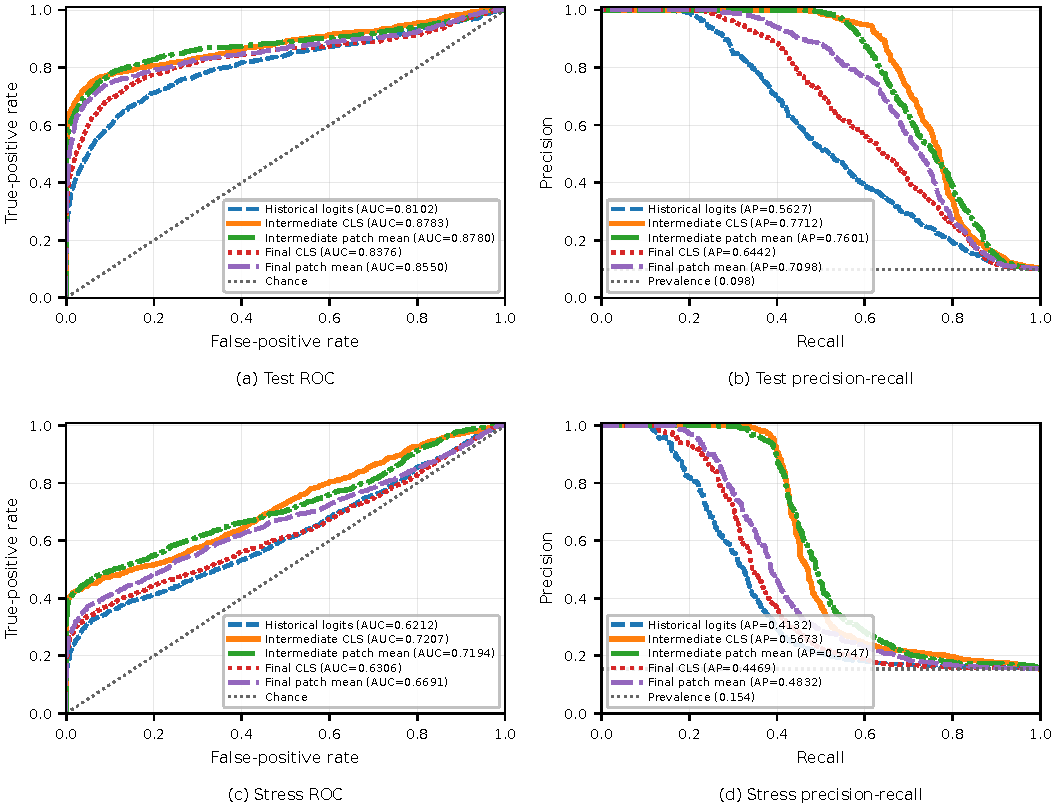
\includegraphics[width=0.99\textwidth]{Figures/vit_ablation_composite_v2_1.pdf}
    \caption{\textcolor{red}{Controlled ViT-B/16 descriptor ablation on KITTI sequence 05: (a) test ROC, (b) test precision--recall, (c) stress ROC, and (d) stress precision--recall. Historical logits denote the two-region classification-logit descriptor recovered from the legacy notebooks; intermediate and final CLS/patch-mean variants are new controlled internal-token ablations. Thresholds were selected by maximum F1 on the calibration split and frozen for test and stress. Ambiguous pairs were excluded from binary evaluation.}}
    \label{fig:vit_descriptor_ablation}
\end{figure*}

\begin{table*}[t]
    \centering
    \caption{\textcolor{red}{Controlled ViT-B/16 descriptor ablation on KITTI sequence 05. The best value in each metric column is shown in bold.}}
    \label{tab:vit_descriptor_ablation}
    {\color{red}
    \setlength{\tabcolsep}{3.5pt}
    \resizebox{\textwidth}{!}{%
    \begin{tabular}{llllcccccc}
        \toprule
        Descriptor & Token source & Pooling & Dim. &
        \multicolumn{3}{c}{Test} &
        \multicolumn{3}{c}{Stress} \\
        \cmidrule(lr){5-7}\cmidrule(lr){8-10}
        & & & & ROC-AUC & AP & F1 & ROC-AUC & AP & F1 \\
        \midrule
        Historical logits & Classification logits & Model output & 2000 &
        0.8102 & 0.5627 & 0.4870 & 0.6212 & 0.4132 & 0.3758 \\
        Intermediate CLS & Block 5 & CLS & 1536 &
        \textbf{0.8783} & \textbf{0.7712} & \textbf{0.7344} &
        \textbf{0.7207} & 0.5673 & \textbf{0.5561} \\
        Intermediate patch mean & Block 5 & Patch mean & 1536 &
        0.8780 & 0.7601 & 0.6960 & 0.7194 &
        \textbf{0.5747} & 0.5508 \\
        Final CLS & Block 11 & CLS & 1536 &
        0.8376 & 0.6442 & 0.5608 & 0.6306 & 0.4469 & 0.4057 \\
        Final patch mean & Block 11 & Patch mean & 1536 &
        0.8550 & 0.7098 & 0.6523 & 0.6691 & 0.4832 & 0.4401 \\
        \bottomrule
    \end{tabular}%
    }
    \vspace{2pt}

    \footnotesize Historical logits preserve the legacy notebook descriptor and matching semantics. Intermediate/final CLS and patch-mean rows are new controlled internal-token ablations. The evaluation is restricted to KITTI sequence 05.
    }
\end{table*}

\FloatBarrier

\raggedbottom

\section{Conclusion and Future Work}
\label{sec:concl}

The experimental results reinforce that viewpoint variations, opposite traversal directions, and camera rotations remain challenging conditions for Loop Closure Detection in Visual SLAM environments.

The proposed framework was used to comparatively evaluate CNN- and Transformer-based visual descriptors using standardized preprocessing and descriptor-matching procedures across the KITTI and TUM datasets. The experiments enabled a comparative assessment of descriptor behavior under stable viewpoints, opposite traversal directions, and camera rotation conditions. Because Loop Closure Detection is an imbalanced classification problem, the analysis emphasized F1-score and AUC in addition to Accuracy, providing a more reliable assessment of descriptor performance. 

The experimental results indicate that descriptor performance varies across operational conditions and representation-learning strategies. Among the evaluated architectures, the Adapted and Fine-Tuned VGG-16 achieved the best performance under relatively stable viewpoint conditions and showed improved descriptor discriminability across the evaluated scenarios. ResNet exhibited improved performance under opposite-traversal conditions, suggesting greater tolerance to changes in traversal direction. The experiments also indicate that camera rotations reduced descriptor consistency, increasing FP and FN rates during descriptor matching and decreasing overall detection reliability.

This work contributes a comparative evaluation framework for Loop Closure Detection in Visual SLAM using CNN- and Transformer-based visual descriptors under unified experimental conditions. The study also provides an experimental analysis of descriptor behavior under viewpoint variation, opposite traversal directions, and camera rotations using the KITTI and TUM datasets. Publicly available datasets, pretrained models, and standardized evaluation metrics were adopted to support reproducibility and future comparative studies.



\begin{revisionblock}
The reproducible KITTI 05 audit also showed that the mathematical definition and implementation of descriptor distance materially affect the reported results. Replacing the reconstructed maximum-component formulation with a flattened Euclidean distance improved AP and fixed-threshold F1-score on calibration, test, and stress events, while the isolated calibration protocol prevented threshold leakage into the final evaluations. This additional experiment strengthens the reproducibility of the framework and establishes a descriptor-level baseline for the subsequent temporal ablation.
\end{revisionblock}

Future work will investigate deploying the proposed framework on physical robotic platforms under varying illumination conditions and camera motion. Additional studies should also evaluate adaptive threshold-selection strategies and omnidirectional imaging systems for improved robustness under opposite traversal conditions. Further investigations may explore self-supervised descriptor learning and multimodal place-recognition approaches for challenging Visual SLAM environments.

Although the proposed operational thresholds produced satisfactory performance in the evaluated scenarios, sensitivity to threshold variation was not systematically analyzed and should be investigated in future studies.

\bibliographystyle{IEEEtran}
% BEGIN KITTI05_SOTA_REFERENCE_COLOR_HOOK
\makeatletter
\let\kittiSotaOriginalBibitem\bibitem
\renewcommand{\bibitem}[2][]{%
  \def\kittiSotaCurrentBibKey{#2}%
  \def\kittiSotaDbowBibKey{GalvezLopez2012DBoW2}%
  \def\kittiSotaNetvladBibKey{Arandjelovic2016NetVLAD}%
  \ifx\kittiSotaCurrentBibKey\kittiSotaDbowBibKey
    \color{red}%
  \else\ifx\kittiSotaCurrentBibKey\kittiSotaNetvladBibKey
    \color{red}%
  \else
    \color{black}%
  \fi\fi
  \if\relax\detokenize{#1}\relax
    \kittiSotaOriginalBibitem{#2}%
  \else
    \kittiSotaOriginalBibitem[#1]{#2}%
  \fi
}
\makeatother
% END KITTI05_SOTA_REFERENCE_COLOR_HOOK
\bibliography{references_revised}
\color{black}

\begin{IEEEbiographynophoto}{Fabiana Naomi Iegawa} received a BSc in Control and Automation Engineering in 2018 from the Mauá School of Engineering (São Caetano do Sul/São Paulo, Brazil) and completed her MSc in Computer Science in 2023 at the Federal University of ABC (UFABC). She has expertise in Control and Automation Engineering, with a focus on EEG-Based Control Systems. Her projects include developing Human-Robot Interaction using Brain-Computer Interfaces (BCI). During her Master's, she worked on SLAM, Image Processing, and Convolutional Neural Networks (CNN) for Loop Closure detection in autonomous robot navigation. She also has experience in Machine Learning Engineering in the financial and retail sectors, with skills in predictive and prescriptive modeling, model governance, and MLOps pipeline design. The author received the Best Student Paper Award at the Information Technology: New Generation (ITNG) in 2024.
\end{IEEEbiographynophoto}

\begin{IEEEbiographynophoto}{Wagner Tanaka Botelho} received a BSc in Computer Engineering from Dom Bosco Catholic University, Campo Grande, Brazil, in 2002; a MSc in Systems and Computer Engineering from the Military Institute of Engineering, Rio de Janeiro, Brazil, in 2005; and a PhD in Information and Science Technology in the Department of Biocybernetics from Niigata University, Japan, in 2009. Currently, he is a professor at the Centre of Mathematics, Computation and Cognition (CMCC), Federal University of ABC, Brazil. His research interests include Mobile Robots, Multi-Robot Systems, Artificial Intelligence, and DNNs.
\end{IEEEbiographynophoto}

\begin{IEEEbiographynophoto}{Flavio Shigeo Yamamoto} holds an undergraduate degree in Mathematics and an MSc in Computer Science from the University of São Paulo. I have worked at universities, teaching and conducting research in Artificial Intelligence and in the links between creative thinking and cross-curricular activities for about 15 years. I am currently Head of Cognitive Robotics at NTU Soft. Tech and Chief Technology Innovation Officer at ANJUNA-TECH and ACCIST. My research focuses on visuospatial cognition and episodic memory. I am exploring how to implement a cognitive architecture for humanoid robots that supports these cognitive mechanisms to facilitate teaming between humans and personal robots (some of which are integrated with LLMs).
\end{IEEEbiographynophoto}

\begin{IEEEbiographynophoto}{Fabio Suim Chagas}
received the B.Sc. degree in Computer Science from the Federal University of Viçosa (UFV), Brazil, in 2001, the M.Sc. degree in Systems and Computing from the Military Institute of Engineering (IME), Brazil, in 2005, and the Ph.D. degree in Defense Engineering from IME, in 2021. From 2021 to 2023, he was a Postdoctoral Researcher with the National Institute for Pure and Applied Mathematics (IMPA), Brazil, where he worked on machine learning, computer graphics, and motion analysis. From 2024 to 2025, he was a Researcher with the University of South-Eastern Norway (USN), contributing to the AI4HyDrop project, focused on a dynamic AI-based framework for safe drone operations in restricted and urban areas. He is currently a Researcher with the Department of Design, Norwegian University of Science and Technology (NTNU), Norway, where he works on the SHEREC project (Safe, Healthy and Environmental Ship Recycling), which develops robotics-, data-, and AI-based solutions to improve occupational safety and environmental sustainability in ship recycling. His research interests include machine learning, robotics, computer graphics, motion analysis, haptics, and kinematic modeling.
\end{IEEEbiographynophoto}

\begin{IEEEbiographynophoto}{Marlon M. L\'{o}pez-Flores} received a B.Sc. degree in Mathematical Engineering from the National Autonomous University of Honduras (2006), a Master's degree in Mechanical Engineering from the State University of Rio de Janeiro (2014), and a PhD in Mechanical Engineering from the State University of Rio de Janeiro (2018). Completed postdoctoral research at the Fluid Dynamics Laboratory (FLUID) of the National Institute of Pure and Applied Mathematics - IMPA (2020-2023). Currently a postdoctoral researcher at the Laboratory of Artificial Intelligence, Robotics and Cybernetics (LIARC) of the Military Institute of Engineering (IME - RJ), focusing on the application of Artificial Intelligence in Mathematical Modeling. His research interests include Applied Mathematics, Numerical Methods, and Mechanics, with an emphasis on Mathematical Modeling in Transport Phenomena.
\end{IEEEbiographynophoto}

\begin{IEEEbiographynophoto}{Paulo Fernando Ferreira Rosa} received a B.Sc. degree in Electrical Engineering from the Federal University of Pernambuco, Brazil, in 1986, a M.Eng. degree in Computer Science and Systems Engineering from the Kyushu Institute of Technology, Japan, in 1994, and a Ph.D. degree in Information Engineering from Niigata University, Japan, in 1997. He has been a tenured professor at the Military Institute of Engineering (IME), Brazil, since 2002, where he is currently a Full Professor and coordinates the Artificial Intelligence, Robotics and Cybernetics Laboratory (LIARC). His research interests include robotics and automation, autonomous mobile robots, flexible manipulators, smart homes, and unmanned aerial vehicles. He currently coordinates and participates in research projects on UAVs and mobile robots funded by official agencies.
\end{IEEEbiographynophoto}

\EOD

\end{document}
